%% 
%% Copyright 2007-2024 Elsevier Ltd
%% 
%% This file is part of the 'Elsarticle Bundle'.
%% ---------------------------------------------
%% 
%% It may be distributed under the conditions of the LaTeX Project Public
%% License, either version 1.3 of this license or (at your option) any
%% later version.  The latest version of this license is in
%%    http://www.latex-project.org/lppl.txt
%% and version 1.3 or later is part of all distributions of LaTeX
%% version 1999/12/01 or later.
%% 
%% The list of all files belonging to the 'Elsarticle Bundle' is
%% given in the file `manifest.txt'.
%% 
%% Template article for Elsevier's document class `elsarticle'
%% with numbered style bibliographic references
%% SP 2008/03/01
%% $Id: elsarticle-template-num.tex 249 2024-04-06 10:51:24Z rishi $
%%
% \documentclass[preprint,12pt]{elsarticle}

%% Use the option review to obtain double line spacing
% \documentclass[authoryear,preprint,review,12pt]{elsarticle}

%% Use the options 1p,twocolumn; 3p; 3p,twocolumn; 5p; or 5p,twocolumn
%% for a journal layout:
%% \documentclass[final,1p,times]{elsarticle}
%% \documentclass[final,1p,times,twocolumn]{elsarticle}
\documentclass[final,3p,times]{elsarticle}
%% \documentclass[final,3p,times,twocolumn]{elsarticle}
%% \documentclass[final,5p,times]{elsarticle}
%% \documentclass[final,5p,times,twocolumn]{elsarticle}

%% For including figures, graphicx.sty has been loaded in
%% elsarticle.cls. If you prefer to use the old commands
%% please give \usepackage{epsfig}

%% The amssymb package provides various useful mathematical symbols
\usepackage{amssymb}
%% The amsmath package provides various useful equation environments.
\usepackage{amsmath}
\usepackage[hidelinks]{hyperref}
\usepackage{algorithmic}
\usepackage{algorithm}
\usepackage{subfigure}
\usepackage{booktabs}
\usepackage{bm}
%%%%%%%%%%%%%%%%%%%%%%%%%%%%%%%%
% THEOREMS
%%%%%%%%%%%%%%%%%%%%%%%%%%%%%%%%
\usepackage{amsthm}
\usepackage[inline, shortlabels]{enumitem}
\theoremstyle{plain}
\newtheorem{theorem}{Theorem}[section]
\newtheorem{proposition}[theorem]{Proposition}
\newtheorem{lemma}[theorem]{Lemma}
\newtheorem{corollary}[theorem]{Corollary}
\theoremstyle{definition}
\newtheorem{definition}[theorem]{Definition}
\newtheorem{assumption}[theorem]{Assumption}
\theoremstyle{remark}
\newtheorem{remark}[theorem]{Remark}

\newcommand{\bE}{\mathbb{E}}
\newcommand{\bR}{\mathbb{R}}
\newcommand{\bS}{\mathbb{S}}
\newcommand{\bU}{\mathbb{U}}
\newcommand{\bK}{\mathbb{K}}
\newcommand{\bV}{\mathbb{V}}
\newcommand{\bP}{\mathbb{P}}

\newcommand{\vmu}{{\boldsymbol \mu}}
\newcommand{\vepsilon}{{\boldsymbol \epsilon}}
\newcommand{\vphi}{{\boldsymbol \phi}}
\newcommand{\vtheta}{{\boldsymbol \theta}}
\newcommand{\vSigma}{{\boldsymbol \Sigma}}

% mathcal type
\newcommand{\hA}{\mathcal{A}}
\newcommand{\hB}{\mathcal{B}}
\newcommand{\hC}{\mathcal{C}}
\newcommand{\hD}{\mathcal{D}}
\newcommand{\hE}{\mathcal{E}}
\newcommand{\hF}{\mathcal{F}}
\newcommand{\hG}{\mathcal{G}}
\newcommand{\hH}{\mathcal{H}}
\newcommand{\hI}{\mathcal{I}}
\newcommand{\hJ}{\mathcal{J}}
\newcommand{\hK}{\mathcal{K}}
\newcommand{\hL}{\mathcal{L}}
\newcommand{\hM}{\mathcal{M}}
\newcommand{\hN}{\mathcal{N}}
\newcommand{\hO}{\mathcal{O}}
\newcommand{\hP}{\mathcal{P}}
\newcommand{\hQ}{\mathcal{Q}}
\newcommand{\hR}{\mathcal{R}}
\newcommand{\hS}{\mathcal{S}}
\newcommand{\hT}{\mathcal{T}}
\newcommand{\hU}{\mathcal{U}}
\newcommand{\hV}{\mathcal{V}}
\newcommand{\hW}{\mathcal{W}}
\newcommand{\hX}{\mathcal{X}}
\newcommand{\hY}{\mathcal{Y}}
\newcommand{\hZ}{\mathcal{Z}}

\newcommand{\bI}{\mathbb{I}}

\newcommand{\vzero}{{\bf 0}}
\newcommand{\vx}{{\bf x}}
\newcommand{\vz}{{\bf z}}
\newcommand{\vc}{{\bf c}}
\newcommand{\vy}{{\bf y}}
\newcommand{\vI}{{\bf I}}
\newcommand{\vd}{{\bf d}}

\DeclareMathOperator*{\argmin}{arg\,min}

\usepackage{amssymb}% http://ctan.org/pkg/amssymb
\usepackage{pifont}% http://ctan.org/pkg/pifont
\newcommand{\cmark}{\ding{51}}%
\newcommand{\xmark}{\ding{55}}%
%% The amsthm package provides extended theorem environments
%% \usepackage{amsthm}

%% The lineno packages adds line numbers. Start line numbering with
%% \begin{linenumbers}, end it with \end{linenumbers}. Or switch it on
%% for the whole article with \linenumbers.
%% \usepackage{lineno}

% 自定义颜色和高亮命令

\usepackage{geometry}
\usepackage{booktabs}
\usepackage{multirow}
\usepackage{xcolor}
\usepackage[normalem]{ulem} % normalem 防止改变 \emph 的默认行为
\usepackage{graphicx}
\definecolor{myblue}{RGB}{0, 112, 192} % 接近图中的蓝色
\newcommand{\best}[1]{\textbf{\textcolor{red}{#1}}}
\newcommand{\second}[1]{\underline{\textit{\textcolor{myblue}{#1}}}}



\journal{Knowledge-Based Systems}

\begin{document}

\begin{frontmatter}

%% Title, authors and addresses

%% use the tnoteref command within \title for footnotes;
%% use the tnotetext command for theassociated footnote;
%% use the fnref command within \author or \affiliation for footnotes;
%% use the fntext command for theassociated footnote;
%% use the corref command within \author for corresponding author footnotes;
%% use the cortext command for theassociated footnote;
%% use the ead command for the email address,
%% and the form \ead[url] for the home page:
%% \title{Title\tnoteref{label1}}
%% \tnotetext[label1]{}
%% \author{Name\corref{cor1}\fnref{label2}}
%% \ead{email address}
%% \ead[url]{home page}
%% \fntext[label2]{}
%% \cortext[cor1]{}
%% \affiliation{organization={},
%%             addressline={},
%%             city={},
%%             postcode={},
%%             state={},
%%             country={}}
%% \fntext[label3]{}

\title{PDT: Predictive Domain Transform for Multivariate Time Series Forecasting}

%% use optional labels to link authors explicitly to addresses:
%% \author[label1,label2]{}
%% \affiliation[label1]{organization={},
%%             addressline={},
%%             city={},
%%             postcode={},
%%             state={},
%%             country={}}
%%
%% \affiliation[label2]{organization={},
%%             addressline={},
%%             city={},
%%             postcode={},
%%             state={},
%%             country={}}

\author{Chenhao Ying}
\ead{chenhying01@zju.edu.cn}
\author{Jiangang Lu\corref{cor1}}
\ead{lujg@zju.edu.cn}
%% Author affiliation
\address{{State Key Laboratory of Industrial Control Technology, College of Control Science and Engineering, Zhejiang University},
            {Hangzhou},
            {310027}, 
            {Zhejiang},
            {China}}



\cortext[cor1]{Corresponding author}

%% Abstract
\begin{abstract}
While linear-based models offer inherent computational efficiency for Multivariate Time-Series Forecasting (MTSF), their limited capacity to represent complex non-linear temporal patterns remains a critical bottleneck. To overcome this, we propose a data-adaptive \textbf{Predictive Domain Transform Method (PDTM)}. Unlike fixed-basis transforms, PDTM projects time series into a prediction-optimal latent space characterized by energy concentration, explicitly minimizing prediction error and alleviating the representation burden on subsequent layers. Building upon this, we introduce \textbf{PDT}, a dual-route architecture comprising a Linear-Route that extrapolates dominant features via Top-K components, and an Encoder-Route that captures complex non-linear dynamics. Furthermore, to address inter-variate dependencies, we propose a \textbf{Masked Channel Dependent (MCD)} strategy implemented via a lightweight Linear-Attention mechanism. MCD employs a distance-based masking strategy to effectively suppress noise from irrelevant channels while enhancing information fusion among strongly correlated variates. Extensive experiments on real-world datasets demonstrate that PDT achieves state-of-the-art performance, achieving a superior balance between forecasting accuracy and computational efficiency.
\end{abstract}

%%Graphical abstract
% \begin{graphicalabstract}
%\includegraphics{grabs}
% \end{graphicalabstract}

%%Research highlights
\begin{highlights}
\item A data-adaptive Predictive Domain Transform Method (PDTM) is proposed to project time series into a prediction-optimal domain, overcoming the limitations of fixed-basis transforms.
\item A dual-route architecture (PDT) leverages energy concentration to effectively extrapolate dominant linear features while capturing complex non-linear dynamics.
\item A Masked Channel Dependent (MCD) strategy with lightweight Linear-Attention is introduced to selectively fuse inter-channel dependencies and suppress noise.
\item PDT achieves state-of-the-art performance on benchmark datasets with exceptional computational efficiency.
\end{highlights}

%% Keywords
\begin{keyword}
%% keywords here, in the form: keyword \sep keyword
Time series forecasting, %conditional diffusion models,
Domain Transform,
Linear model,
Channel dependent.
%% PACS codes here, in the form: \PACS code \sep code

%% MSC codes here, in the form: \MSC code \sep code
%% or \MSC[2008] code \sep code (2000 is the default)

\end{keyword}

\end{frontmatter}

%% Add \usepackage{lineno} before \begin{document} and uncomment 
%% following line to enable line numbers
%% \linenumbers

%% main text

%% Use \section commands to start a section
\section{Introduction}

Time-series forecasting (TSF) plays a pivotal role across a wide range of application domains, serving as a foundation for decision-making\cite{carli2020iot,wang2020controllability}. In real-world scenarios, systems are typically characterized by the co-evolution of multiple coupled variables, making Multivariate Time-Series Forecasting (MTSF) significantly more challenging than its univariate counterpart\cite{stock2001vector,lim2021temporal}. Predicting a target variable necessitates modeling both the influence from other variables and temporal dependencies. Thus, two primary challenges emerge: robustly capturing long-term temporal correlations and effectively disentangling complex inter-variable dependencies.

In recent years, Transformer-based and Linear-based models have emerged as two dominant paradigms. While Transformers initially dominated the field due to their global interaction capabilities\cite{zhou2021informer,wu2021autoformer,piao2024fredformer,liu2022non,cirstea2022triformer}, the emergence of simple linear models (e.g., DLinear\cite{zeng2023transformers}) has challenged their mainstream, demonstrating that linear mappings can achieve comparable or superior accuracy with significantly lower computational overhead. A consensus suggests that Linear models excel in series with stable trends, whereas Transformers offer superior feature extraction for complex dynamics\cite{li2023revisiting}. Despite their efficiency, Linear-based models face a bottleneck in representing complex non-linear temporal patterns, necessitating advanced domain transformation techniques.

To overcome the limitations of time-domain linear mappings, frequency-domain transforms have been introduced. Methods like FreTS\cite{yi2023frequency} and FITS\cite{xu2024fits} leverage Fourier\cite{bloomfield2004fourier} or Wavelet transforms\cite{grossmann1984decomposition} to map signals into a semantically informative representation, alleviating the representation burden on linear layers\cite{sasal2022w}. However, these approaches rely on \textit{fixed-basis} transforms (e.g., Fourier or Wavelet bases), which are data-agnostic. This rigidity limits their adaptability to diverse datasets with varying spectral characteristics, potentially leading to suboptimal feature representation. 

To address the limitations of fixed bases, we propose a data-adaptive \textbf{Predictive Domain Transform Method(PDTM)}. Unlike fixed transforms, PDTM learns a basis specifically optimized to minimize prediction error, projecting input segments into a "prediction-optimal" latent space. We experimentally demonstrate that PDTM exhibits an energy concentration property\cite{yi2023frequency} similar to frequency transforms, but with greater flexibility. Based on this, we introduce \textbf{PDT}, a lightweight linear forecasting framework built upon the learnable PDTM and a Dual-Route architecture. It employs a Linear-Route to extrapolate the dominant, linearly predictable components and a parallel Encoder-Route to capture residual complex non-linear dynamics, effectively raising the performance ceiling while maintaining the efficiency of linear models. 

Modeling inter-series dependencies is another critical challenge\cite{wang2020deep}. Existing methods generally fall into Channel-Independent (CI) or Channel-Dependent (CD) paradigms\cite{luo2025adapformer}. Although CI approaches (e.g. PatchTST\cite{nie2023a}) avoid channel noise by treating channels independently, they discard valuable cross-variable information. Conversely, CD approaches (e.g., iTransformer\cite{liu2024itransformer}) capture global dependencies, but are prone to overfitting spurious correlations in high-dimensional multivariate systems. To bridge this gap, we propose a \textbf{Masked Channel Dependent (MCD)} strategy. Instead of treating all channels uniformly, MCD utilizes a learnable mask based on distance metrics to selectively fuse information from strongly correlated variates while suppressing irrelevant noise. Furthermore, we implement a lightweight Linear-Attention (LA) mechanism to achieve this fusion efficiently, avoiding the high computational cost of traditional attention\cite{Vaswani2017_atten}.

The contributions of the work are summarized as follows:

\begin{enumerate}[\indent 1)]
\item We introduce a data-adaptive Predictive Domain Transform Method (PDTM) optimized for minimum forecast error, which substantially alleviates the representation burden on Linear-based models. We further demonstrate that PDTM exhibits energy concentration properties comparable to frequency-domain transforms, which facilitates lightweight design and noise suppression.
\item Leveraging the properties of PDTM, we propose a linear-based dual-route architecture, PDT. The architecture introduces a learnable PDTM and a Spectrum-fix embedding for feature encoding, while further employs parallel Linear-Route and Encoder-Route to process linearly predictable features and complex nonlinear features respectively.
\item We introduce a novel Masked Channel Dependent (MCD) strategy for channel-wise dependency fusion, which employs a learnable mask constructed from distance metrics to suppress noise from irrelevant channels while enhancing sensitivity to dependencies among correlated channels. In addition, we implement attention in a lightweight and linearized form to reduce both computational and memory costs.
\item Extensive experiments on multiple real-world datasets show that proposed PDT achieves state-of-the-art performance. Resource profiling confirms that our model achieves an exceptional trade-off between computational efficiency and performance.
\end{enumerate}


\section{Related Work}

\subsection{MTSF model Architecture}

Time series forecasting (TSF) has long been a central topic in statistics and data science. Classical statistical methods, including ARIMA\cite{box2015time}, exponential smoothing\cite{gardner1985exponential}, and spectral analysis\cite{koopmans1995spectral}, have served as primary tools for a long time. With the development of artificial intelligence, deep learning has fundamentally advanced time series forecasting (TSF). Early sequence modeling relied on Recurrent Neural Networks (RNNs)\cite{yu2019review,salinas2020deepar} and Temporal Convolutional Networks (TCNs)\cite{bai2018empirical, wu2023timesnet}. However, these architectures often struggle with capturing ultra-long-term dependencies or incur high computational costs. Consequently, Transformer-based models became mainstream, leveraging self-attention to model global dependencies\cite{wen2023trans}. Approaches like Informer\cite{zhou2021informer} and Autoformer~\cite{wu2021autoformer} introduced sparse attention and decomposition mechanisms to enhance efficiency. Despite their success, the necessity of complex attention mechanisms was challenged by DLinear\cite{zeng2023transformers}, which achieved comparable performance using simple linear layers. This prompted a shift towards refined architectures: PatchTST\cite{nie2023a} introduced patch-wise tokenization to capture local semantics, while iTransformer\cite{liu2024itransformer} proposed inverting dimensions to apply attention across variates. Crossformer\cite{zhang2023crossformer} and TFEformer\cite{ying2024tfeformer} further realize two-dimensional dependency modeling by combining intra-series patch segmentation with inter-variate attention, thereby capturing both temporal-wise and variate-wise dependencies. Recent linear-based variants, such as N-BEATS\cite{oreshkin2019n} and TimeMixer\cite{wang2024timemixer}, further explored interpretability and multi-scale modeling. However, a critical limitation remains: pure linear-based models inherently lack the capacity to represent complex non-linear dynamics, while heavy Transformer architectures are computationally expensive. Our PDT addresses this by integrating a data-adaptive transform to handle non-linearity within an efficient dual-route linear framework.

\subsection{Domain Transform}

To alleviate the representation bottleneck\cite{nie2023a} of the time domain, projecting series into a latent space has proven effective. Classical approaches utilize fixed bases, such as Fourier or Wavelet transforms, to exploit spectral sparsity. FreTS\cite{yi2023frequency} and FITS\cite{xu2024fits} demonstrate that mapping time-domain signals to the frequency domain allows lightweight MLPs to capture global patterns efficiently. Similarly, FilterNet\cite{yi2024filternet} employs learnable filters to selectively preserve spectral components. However, these methods rely on \textit{fixed} or \textit{generic} bases (e.g. DFT), which are agnostic to the specific prediction task or dataset. While recent works like FreDF\cite{wang2025fredf} and TransDF\cite{wang2025transdf} began to explore dataset-adaptive decorrelation transform, they focus on mitigating autocorrelation rather than explicitly optimizing for prediction accuracy. Our work goes further by proposing a Predictive Domain Transform Method (PDTM). Instead of using a predefined basis, PDTM learns a dataset-specific basis that explicitly maximizes the "predictability" of the projected domain, concentrating the most valuable forecasting information into the principal components.


\subsection{Channel-dependent Strategy}
Modeling inter-variate correlations is a core challenge in MTSF, generally categorized into Channel-Independent (CI) and Channel-Dependent (CD) paradigms. The CI paradigm, exemplified by PatchTST\cite{nie2023a} and most linear models\cite{zeng2023transformers, xu2024fits, yi2024filternet}, treats variates independently to avoid channel-wise noise overfitting, offering robustness but sacrificing cross-variate information. Conversely, the CD paradigm explicitly models interactions. iTransformer\cite{liu2024itransformer} and Crossformer\cite{zhang2023crossformer} leverage attention mechanisms to capture cross-channel dependencies, while SOFTS\cite{han2024softs} employs a STAR (STar Aggregate and Redistribute) aggregate module to performs a centralized aggregation and redistribution of cross-channel dependencies. However, treating all channels uniformly is suboptimal under both CI and CD. To bridge this gap, we propose a Masked Channel Dependent (MCD) strategy. Unlike rigid CI or CD, MCD utilizes a distance-based learnable mask to selectively fuse information only from strongly correlated variates, achieving a balance between information utilization and noise suppression.


\section{Methodology}

\subsection{Problem Definition}

In the data-driven approaches, multivariate time series forecasting is formulated as mapping multivariate historical observations to future values over a single-step or multi-step horizon. Formally, let $X=[x_1,x_2,...,x_T]\in \mathbb{R}^{N \times T}$ represent the multivariate time series, where $x_t \in \mathbb{R}^N$ denotes the observation of $N$ variates at time step $t$. Given a historical window of length $L$, $X_{t-L+1:t}=[x_{t-L+1},x_{t-L+2},...,x_{t}]$, the objective of MTSF is to forecast the future values for the next $T$ time steps, represented as $\hat{X}_{t+1:t+T} = [\hat{x}_{t+1},\hat{x}_{t+2},...,\hat{x}_{t+T}]$. The forecasting model is represented as a learnable parametric function $\mathcal{F}(\Theta)$, and the overall process can be written as:
\begin{align}
\label{eqn_fore}
\hat{X}_{t+1:t+T}=\mathcal{F}(X_{t-L+1:t};\Theta)
\end{align}
where $\Theta$ denotes the learnable parameters of the model. During training, the objective is to minimize the forecasting error, measured by the $L2$ norm between the predicted values $\hat{X}_{t+1:t+T}$ and the ground truth $X_{t+1:t+T}$. The loss function is given by:
\begin{align}
\label{eqn_foreloss}
\mathcal{L}(\Theta)=\frac{1}{T}\sum_{i=t+1}^{t+T}{||\hat{x}_i-x_i||^2}
\end{align}


\subsection{Predictive Domain Transform Method}
\label{sec:pdt}

To overcome the representation bottleneck of linear models and the rigidity of fixed-basis transforms, we introduce the \textbf{Predictive Domain Transform Method (PDTM)}. Unlike generic transforms that focus on signal reconstruction or frequency sparsity, PDTM is mathematically derived to project time-domain series into a latent subspace explicitly optimized for minimizing future forecasting error.

\subsubsection{Formulation and Optimization Objective}

Let $\mathbf{x} \in \mathbb{R}^{L}$ denote the historical look-back window and $\mathbf{y} \in \mathbb{R}^{T}$ denote the future horizon to be predicted. We aim to learn a linear transform matrix $\mathbf{B} \in \mathbb{R}^{L\times r}$ that maps the input into a lower-dimensional predictive domain ($r < \min(L,T)$), and a subsequent simplest linear mapping $\mathbf{G} \in \mathbb{R}^{r\times T}$ that makes the prediction from this domain.

The optimization objective is to minimize the Frobenius norm of the prediction error:
\begin{equation}
\label{eqn_pdt_obj}
\min_{\mathbf{B}, \mathbf{G}} \mathbb{E} \left[ \|\mathbf{y} - \mathbf{G}^\top \mathbf{B}^\top \mathbf{x} \|_F^2 \right]
\end{equation}
where $\mathbb{E}[\cdot]$ denotes the expectation over the data distribution. The work of TimeBase\cite{huang2025timebase} has shown that time series data often exhibit similarity in temporal patterns and a low-rank structure. Motivated by this, we employ this formulation essentially seeks a low-rank approximation of the predictive relationship. The low-rank constraint ($r$) forces the model to distill the most salient features governing the transition from past to future, thereby filtering out noise and promoting compact representation.

\subsubsection{Closed-form Solution}

To solve Eq. (\ref{eqn_pdt_obj}), we first define the representation in the predictive domain as $\mathbf{z} = \mathbf{B}^\top \mathbf{x} \in \mathbb{R}^r$. For a fixed basis $\mathbf{B}$, the optimal prediction head $\mathbf{G}$ is the standard least-squares solution. Let $\Sigma_{xx} = \mathbb{E}[\mathbf{x}\mathbf{x}^\top]$ and $\Sigma_{xy} = \mathbb{E}[\mathbf{x}\mathbf{y}^\top]$ denote the covariance and cross-covariance matrices, respectively. The optimal $\mathbf{G}$ is given by:
\begin{equation}
\label{eqn_pdt_Gb}
\mathbf{G}^*(\mathbf{B}) = (\mathbf{B}^\top \Sigma_{xx} \mathbf{B})^{-1} \mathbf{B}^\top \Sigma_{xy}
\end{equation}
To eliminate scaling and rotation ambiguities and ensure a well-conditioned latent space, we impose a \textbf{whitened orthogonality} constraint on the transform basis: $\mathbf{B}^\top \Sigma_{xx} \mathbf{B} = \mathbf{I}_r$. This constraint, commonly used in Canonical Correlation Analysis (CCA), ensures that the transformed features are decorrelated and have unit variance. And prior work\cite{wang2025transdf} has also shown that operating in an orthogonalized (whitened) subspace benefits decorrelation domain forecasting. Under this constraint, Eq. (\ref{eqn_pdt_Gb}) simplifies to: $\mathbf{G}^*(\mathbf{B}) = \mathbf{B}^\top \Sigma_{xy}$.

Substituting $\mathbf{G}^*$ back into Eq. (\ref{eqn_pdt_obj}) and utilizing the cyclic property of the trace, the minimization of error transforms into a trace maximization problem:
\begin{equation}
\label{eqn_pdt_max}
\min_{\mathbf{B}, \mathbf{G}} \text{Error} \iff \max_{\mathbf{B}^\top \Sigma_{xx} \mathbf{B} = \mathbf{I}_r} \operatorname{tr}\left (\mathbf{B}^\top \Sigma_{xy} \Sigma_{yx} \mathbf{B}\right)
\end{equation}
To solve this constrained maximization, we re-parameterize $\mathbf{B}$ as $\mathbf{B} = \Sigma_{xx}^{-1/2} \mathbf{W}$, where $\mathbf{W}$ is an orthogonal matrix such that $\mathbf{W}^\top \mathbf{W} = \mathbf{I}_r$. The problem is then reformulated as:
\begin{equation}
\label{eqn_pdt_tr}
\max_{\mathbf{W}^\top \mathbf{W} = \mathbf{I}_r} \operatorname{tr}(\mathbf{W}^\top \mathbf{H} \mathbf{W}), \quad \text{where} \quad \mathbf{H} \triangleq \Sigma_{xx}^{-1/2} \Sigma_{xy} \Sigma_{yx} \Sigma_{xx}^{-1/2}
\end{equation}
This is a standard eigenvalue problem. We formalize the solution in the following proposition:
\begin{proposition}[Optimal Predictive Domain Basis]
The optimal transform basis $\mathbf{B}^*$ that minimizes the forecasting error consists of the generalized eigenvectors of the predictive covariance matrix. Specifically:
\begin{equation}
\mathbf{B}^* = \Sigma_{xx}^{-1/2} \mathbf{U}_r, \quad \mathbf{G}^* = \mathbf{U}_r^\top \Sigma_{xx}^{-1/2} \Sigma_{xy}
\end{equation}
where $\mathbf{U}_r$ contains the top- $r$ eigenvectors of matrix $\mathbf{H}$ corresponding to the largest eigenvalues.
\end{proposition}

\subsubsection{Energy Concentration and Implementation}

\textbf{Predictability Energy Concentration.} The eigenvalues $\lambda_i(\mathbf{H})$ derived from the trace maximization problem serve as a quantitative metric for the \textit{predictability energy} of each component. As illustrated in Fig.\ref{fig:energy_spectrum}, the energy spectrum across multiple real-world datasets exhibits a sharp decay, indicating that the majority of linearly predictable information is concentrated within the leading top-$K$ directions. 
This phenomenon reveals the core advantage of PDTM: unlike time-domain representations where semantic information is sparsely scattered across $L$ time steps, PDTM compresses the "future-relevant" modes, which typically require complex dependencies to characterize, into a few principal components. This creates a low-dimensional yet semantically dense representation, providing a solid theoretical justification for the \textbf{Top-K} lightweight design in our Linear-Route. By filtering out the tail components corresponding to low eigenvalues, PDTM effectively acts as a denoising filter that preserves only the robust predictive patterns.
\begin{figure}[t]
    \centering
    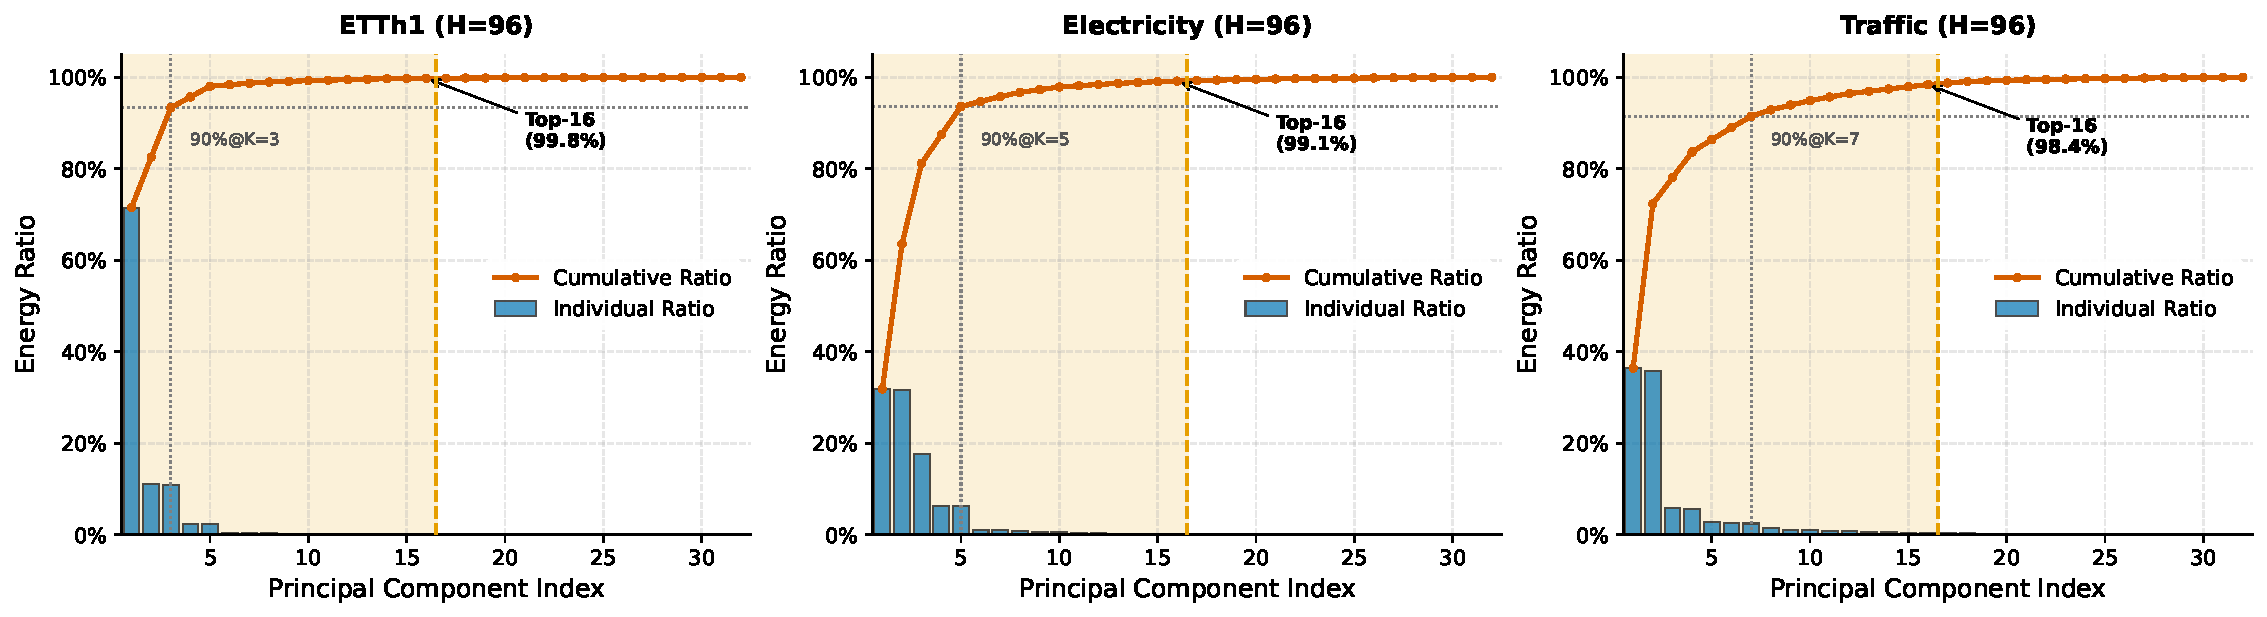
\includegraphics[width=1.0\linewidth]{energy.pdf}
    \caption{\textbf{Predictability Energy Spectrum of PDTM.} The bars represent the normalized energy (eigenvalues) of individual components, and the line indicates the cumulative energy ratio. The shaded area highlights the Top-$K$ components ($K=16$).}\label{fig:energy_spectrum}
\end{figure}


\textbf{Data-Adaptive Implementation.} Unlike fixed-basis transforms (e.g., DFT or Wavelet), PDTM is inherently \textbf{data-adaptive}. The optimal basis $\mathbf{B}^*$ is learned specifically for each dataset to capture its unique correlation structure. The calculation process is outlined in \textbf{Algorithm \ref{alg:pdt_computation}}. Specifically, we employ a sliding window strategy on the training set to construct sample pairs $(\mathbf{x}, \mathbf{y})$ and accumulate the covariance statistics ($\Sigma_{xx}, \Sigma_{xy}$). To ensure numerical stability and handle potential ill-conditioning of covariance matrices, we apply Ridge regularization during the computation:
\begin{equation}
\tilde{\Sigma}_{xx} = \Sigma_{xx} + \alpha \mathbf{I}, \quad (\alpha > 0)
\label{eqn_pdt_ridge}
\end{equation}
This offline-computed basis $\mathbf{B}^*$ serves as a strong prior for the model. In the PDT architecture, we utilize the pre-computed $\mathbf{B}^*$ to initialize the domain transform. We further introduce a learnable adaptation layer to fine-tune these statistics-based priors during end-to-end training, compensating for distribution shifts between the offline statistics and batch-level dynamics.

\begin{algorithm}[t]
\caption{Computation of Data-Adaptive Predictive Domain Transform Method(PDTM)}
\label{alg:pdt_computation}
    \renewcommand{\algorithmicrequire}{\textbf{Input:}} 
    \renewcommand{\algorithmicensure}{\textbf{Output:}}
    \begin{algorithmic}[1]
        \REQUIRE Multivariate time series dataset $\mathcal{D} = \{\mathbf{X}^{(n)}\}_{n=1}^N$, 
                 look-back window $L$, prediction horizon $T$, 
                 reduced rank $r$, Ridge regularization coefficient $\alpha$;
        \ENSURE Optimal transform basis $\mathbf{B}^* \in \mathbb{R}^{L \times r}$, 
                linear prediction head $\mathbf{G}^* \in \mathbb{R}^{r \times T}$;
        
        \STATE \textbf{Initialize:} Covariance matrices $\mathbf{S}_{xx} \leftarrow \mathbf{0}_{L \times L}$, $\mathbf{S}_{xy} \leftarrow \mathbf{0}_{L \times T}$, total samples $M_{total} \leftarrow 0$;
        
        \STATE \textit{// Step 1: Accumulate Statistics (Sample-level)}
        \FOR{each series $\mathbf{X}^{(n)}$ in $\mathcal{D}$}
            \STATE Normalize $\mathbf{X}^{(n)}$ via Z-score;
            \STATE Construct sliding windows: input $\mathbf{x}_i \in \mathbb{R}^L$, target $\mathbf{y}_i \in \mathbb{R}^T$;
            \FOR{each window pair $(\mathbf{x}_i, \mathbf{y}_i)$}
                \STATE $\mathbf{S}_{xx} \leftarrow \mathbf{S}_{xx} + \mathbf{x}_i \mathbf{x}_i^\top$;
                \STATE $\mathbf{S}_{xy} \leftarrow \mathbf{S}_{xy} + \mathbf{x}_i \mathbf{y}_i^\top$;
                \STATE $M_{total} \leftarrow M_{total} + 1$;
            \ENDFOR
        \ENDFOR
        
        \STATE \textit{// Step 2: Compute Population Covariances with Regularization}
        \STATE $\Sigma_{xx} \leftarrow \frac{1}{M_{total}} \mathbf{S}_{xx}$; \quad $\Sigma_{xy} \leftarrow \frac{1}{M_{total}} \mathbf{S}_{xy}$;
        \STATE $\tilde{\Sigma}_{xx} \leftarrow \Sigma_{xx} + \alpha \mathbf{I}_L$; \quad \textit{// Apply Ridge regularization (Eq. \ref{eqn_pdt_ridge})}
        
        \STATE \textit{// Step 3: Solve Trace Maximization via SVD}
        \STATE Compute whitened matrix: $\mathbf{W} \leftarrow \tilde{\Sigma}_{xx}^{-1/2}$ via eigen-decomposition;
        \STATE Construct correlation target matrix: $\mathbf{A} \leftarrow \mathbf{W} \Sigma_{xy}$;
        \STATE Perform Singular Value Decomposition: $\mathbf{U}, \mathbf{\Sigma}, \mathbf{V}^\top = \text{SVD}(\mathbf{A})$;
        \STATE Select Top-$r$ components: $\mathbf{U}_r \leftarrow \mathbf{U}[:, :r]$;
        
        \STATE \textit{// Step 4: Construct Optimal Basis and Head (Proposition 1)}
        \STATE $\mathbf{B}^* \leftarrow \mathbf{W} \mathbf{U}_r$; \quad \textit{// The projection basis}
        \STATE $\mathbf{G}^* \leftarrow \mathbf{U}_r^\top \mathbf{A}$; \quad \textit{// The optimal linear mapping}
        
        \RETURN $\mathbf{B}^*, \mathbf{G}^*$.
    \end{algorithmic}
\end{algorithm}


\subsection{PDT Architecture}

\subsubsection{Overview}

Building upon the theoretical foundation of the Predictive Domain Transform, we propose \textbf{PDT}, a dual-route architecture designed to balance efficiency and capacity. As formally defined in Eq.(\ref{eqn_fore}), the model $\mathcal{F}(\Theta)$ processes a multivariate time series $\mathbf{X} \in \mathbb{R}^{N \times L}$, and the structure is illustrated in Fig.\ref{fig:overview}(a).
To mitigate non-stationarity, we first apply a \textbf{RevIN} (Reversible Instance Normalization) layer. The normalized series is then projected into the prediction-optimal domain (P-Domain) via a learnable PDTM layer.
Leveraging the energy concentration property, the architecture splits into two parallel pathways: (1) a \textbf{Linear-Route} that efficiently extrapolates the dominant Top-$K$ spectral components to capture the main trend; and (2) an \textbf{Encoder-Route} that utilizes full-spectrum information to model complex inter-variate dependencies and non-linear residuals. The dual representations are inversely transformed and fused to generate the final forecast $\hat{\mathbf{Y}}$. The forward process is summarized as:
\begin{equation}
\begin{aligned}
    \mathbf{X}^{\text{Emb}} &= \text{Embed}(\text{PDTM}(\text{RevIN}(\mathbf{X}))) \\
    \mathbf{X}^{\text{Lin}} &= \text{LinearRoute}(\text{TopK}(\mathbf{X}^{\text{Emb}})) \\
    \mathcal{M} &= \text{MaskGen}(\mathbf{X}^{\text{Emb}}) \\
    \mathbf{X}^{\text{Enc}} &= \text{EncoderRoute}(\mathbf{X}^{\text{Emb}}, \mathcal{M}) \\
    \hat{\mathbf{Y}} &= \text{Denorm}(\text{TempMLP}(\mathbf{X}^{\text{Lin}} + \alpha \mathbf{X}^{\text{Enc}}))
\end{aligned}
\end{equation}

\begin{figure}[t]
    \centering
    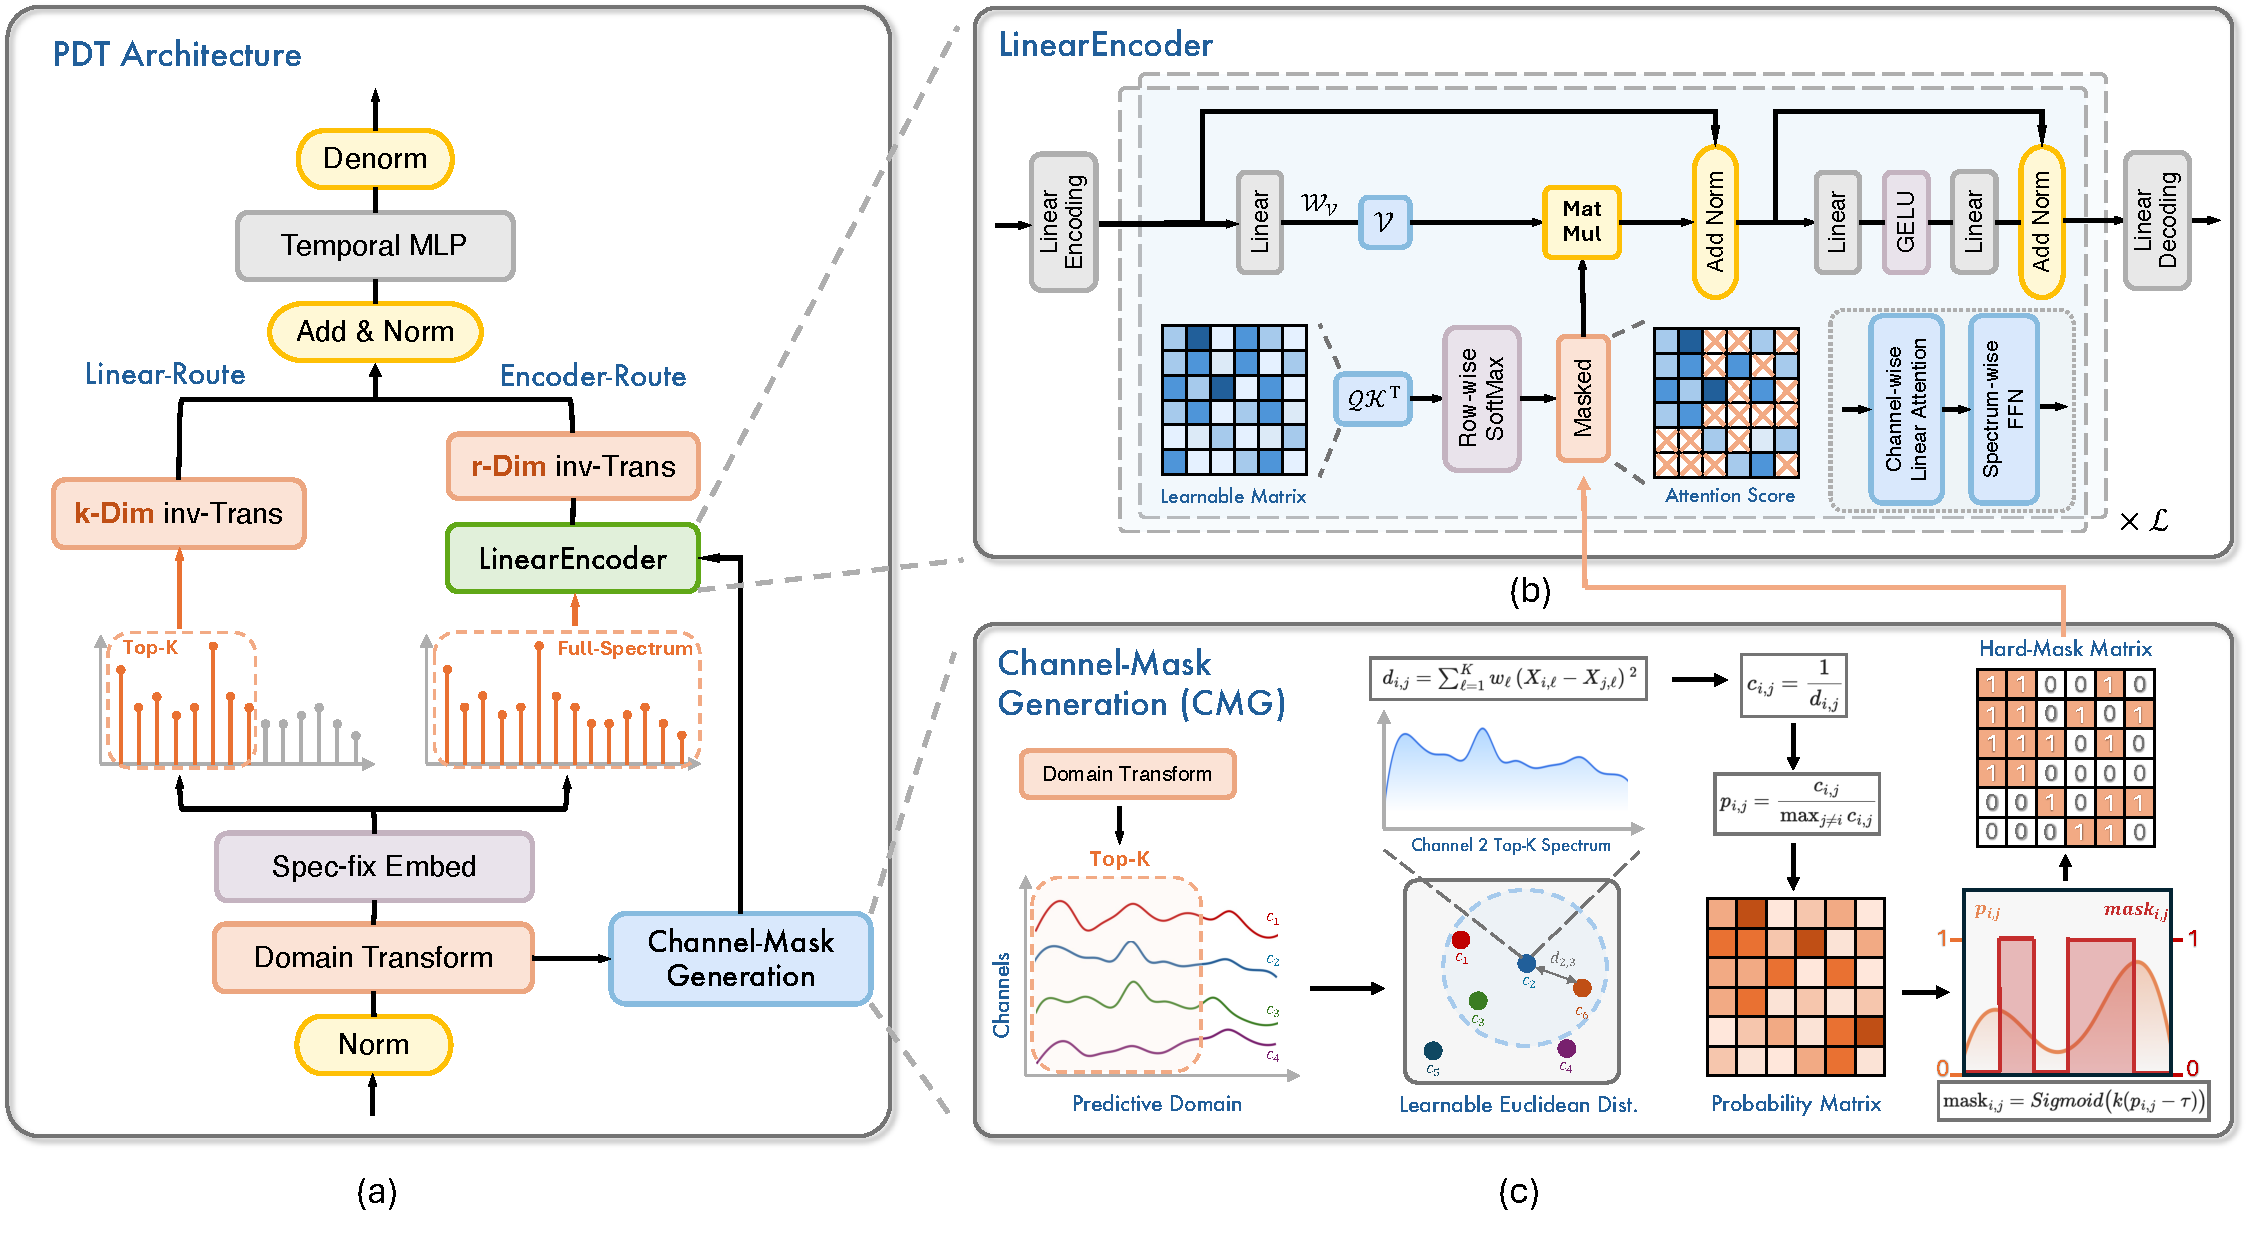
\includegraphics[width=1.0\linewidth]{overview.pdf}
    \caption{\textbf{Overview of the proposed PDT architecture.} 
    \textbf{(a)} The overall framework with dual-route design. 
    \textbf{(b)} The \textit{LinearEncoder} module replaces traditional attention with a lightweight Linear Attention.
    \textbf{(c)} The \textit{Channel Mask Generation (CMG)} module. It computes a learnable Euclidean distance based on the energy-concentrated Top-$K$ components to generate a binary-like hard mask. }\label{fig:overview}
\end{figure}

\subsubsection{Learnable Domain Transform and Embedding}
The Domain Transform layer serves as the bridge between the time domain and the latent P-Domain. While the offline-computed basis $\mathbf{B}^*$ (from Sec.~\ref{sec:pdt}) provides a statistically optimal initialization, it may not fully capture batch-specific variations. Therefore, we define the transform matrix as a learnable parameter $\mathbf{W}_B = \mathbf{B}^* + \mathbf{\Delta}_B$. To preserve the theoretical properties of the P-Domain, we impose an $\ell_\infty$ -norm constraint on the residual: $\|\mathbf{\Delta}_B\|_\infty \le \epsilon$.
The normalized input $\mathbf{X}_{\text{norm}}$ is mapped to the P-Domain via $\mathbf{X}^{P} = \mathbf{X}_{\text{norm}} \mathbf{W}_B \in \mathbb{R}^{N \times r}$.

Subsequently, we introduce a \textbf{Spectrum-fix Embedding}. Unlike temporal embeddings that mix time steps (potentially disrupting the orthogonality of the P-Domain), our embedding expands the feature dimension $D$ while preserving the structural integrity of the $r$ spectral components, as shown in Fig.\ref{fig:embedding}. This yields the embedded tensor $\mathbf{X}^{\text{Emb}} \in \mathbb{R}^{N \times r \times D}$.
Correspondingly, an Inverse Transform layer is deployed at the end of both routes. It utilizes a learnable matrix $\mathbf{W}_G \in \mathbb{R}^{r \times T}$, initialized by the optimal predictor $\mathbf{G}^*$, to project latent features back to the time domain.

\begin{figure}[t]
    \centering
    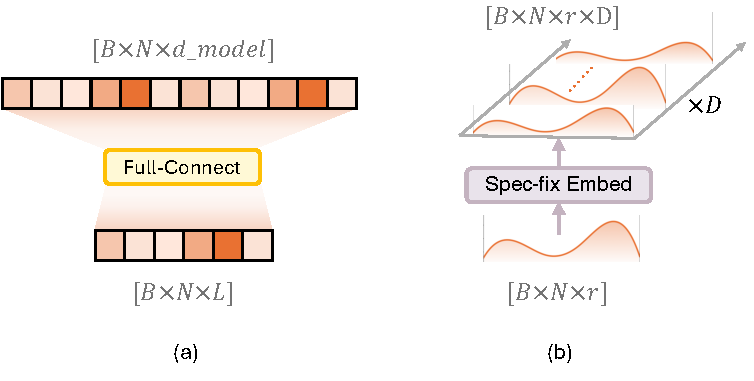
\includegraphics[width=0.5\linewidth]{embedding.pdf}
    \caption{\textbf{Comparison of embedding strategies.} \textbf{(a)} Traditional time-domain embedding mixes temporal information via fully connected layers. \textbf{(b)} Proposed \textit{Spectrum-fix Embedding} expands feature dimensions element-wise, preserving the structural integrity and orthogonality of the P-Domain components.}
    \label{fig:embedding}
\end{figure}

\subsubsection{Linear-Route}
The \textbf{Linear-Route} is designed for extreme efficiency and robustness, grounded in our finding that the majority of linearly predictable energy is concentrated in the leading spectral components. This route extrapolates only the \textbf{Top- $K$} components ($K < r$), acting as a low-pass filter that captures the robust trend while ignoring high-frequency noise.
\begin{equation}
    \mathbf{X}^{\text{Lin}} = \text{TopK}(\mathbf{X}^{\text{Emb}}) \mathbf{W}_G[1: K, :] + \mathbf{b} \quad \in \mathbb{R}^{N \times T \times D}
\end{equation}
where $\mathbf{W}_G$ serves dual roles: linear mapping and inverse transformation. This concise design prevents overfitting and ensures the model's robustness, providing a solid performance baseline.

\subsubsection{Masked Channel Dependent Strategy}
To address the limitations of Channel-Independent (CI) and full Channel-Dependent (CD) paradigms, we propose the \textbf{Masked Channel Dependent (MCD)} strategy. MCD employs a Channel Mask Generation (CMG) module to generate a inter-channel mask which dynamically filter out irrelevant inter-variate interactions, guiding the model to focus on sparse, meaningful couplings. 

\textbf{Channel Mask Generation (CMG).} The specific structure of the CMG module is presented in Fig.\ref{fig:overview}(c). Operating in the P-Domain, CMG computes a learnable similarity metric. Crucially, it utilizes only the Top-$K$ components to reduce computational cost. The distance between channel $i$ and $j$ is defined as a weighted Euclidean distance:
\begin{equation}
    D_{i, j} = \sum_{\ell=1}^{K} w_\ell (X_{i,\ell} - X_{j,\ell})^2, \quad \mathbf{D} = [d_{i, j}] \in \mathbb{R}^{N \times N}
\end{equation}
where $\{w_\ell\}$ are learnable weights governing the importance of each spectral component. The distance matrix $\mathbf{D}$ is converted into a probability matrix $\mathbf{P}$ via inversion and Min-Max normalization. To achieve robust feature selection, we apply a \textit{Threshold-Sigmoid} function to $\mathbf{P}$, generating a binary-like mask $\mathcal{M}$:
\begin{equation}
    M_{i, j} = \sigma\left (k \cdot (p_{i, j} - \tau)\right), \quad \mathcal{M} = [m_{i, j}] \in \mathbb{R}^{N \times N}
\end{equation}
where $\sigma$ is the sigmoid function, $k$ controls steepness, and $\tau$ is the threshold. This differentiable gating mechanism effectively suppresses noise from weakly correlated channels.

\subsubsection{Encoder-Route: LinearEncoder}
The Encoder-Route is designed to capture complex non-linear dynamics and refine inter-channel dependencies. To achieve this, the \textbf{LinearEncoder} adopts a decoupled design: it comprises a Channel-wise Linear Attention module for modeling cross-variate interactions and a Spectrum-wise Feed-Forward Network (FFN) for intra-variate feature evolution, as illustrated in Fig.\ref{fig:overview}(b).

\textbf{Linear Attention (LA)}. Standard multi-head self-attention mechanisms (MHSA) are computationally expensive and are often prone to overfitting in TSF tasks. We propose a lightweight alternative rooted in the inductive bias that, unlike temporal dependencies which shift rapidly, \textit{inter-channel correlations tend to exhibit long-term stability} (e.g., the structural topology between sensors). Consequently, we employ a \textbf{static learnable matrix} $\mathbf{M}_{\text{corr}} \in \mathbb{R}^{N \times N}$ to approximate these global dependencies to replace the process of computing $QK\top$ in the traditional attention mechanism.
To prevent the static parameter from becoming a rigid bottleneck, we inject instance-specific information via the dynamic mask $\mathcal{M}$ generated by the CMG module. This allows the mechanism to combine global structural priors with local adaptive filtering. The attention process is formulated as:
\begin{equation}
\begin{aligned}
    \mathbf{V} &= \mathbf{X}^c \mathbf{W}_v \\
    \mathbf{A} &= \text{Softmax}_{\text{row}}(\mathbf{M}_{\text{corr}} \odot \mathcal{M}) \\
    \mathbf{X}^{\text{chan}} &= \text{Norm}(\mathbf{A} \mathbf{V} + \mathbf{X}^c)
\end{aligned}
\end{equation}
This design reduces the computational complexity while maintaining robust representation capacity (see complexity analysis in Table \ref{table:compl}). 
Subsequently, a \textbf{Spectrum-wise FFN} is applied to model non-linear intra-series dependencies. Operating independently on each channel, it consists of two linear layers with a GELU activation, formulated as $\mathbf{X}^{\text{ctx}} = \text{Norm}(\mathbf{X}^{\text{chan}} + \text{Linear}(\sigma(\text{Linear}(\mathbf{X}^{\text{chan}}))))$, ensuring deep feature extraction across the spectral dimension.

\begin{table}[!t]\small
\centering
\caption{Complexity Analysis of Linear Attention and MHSA}
% \vskip -.1in
\begin{tabular}{c c c}
    \toprule
    Module & Linear Attn & MHSA \\
    \midrule
    FLOPs   & $\mathcal{O}(N^2D+2ND^2)$ & $\mathcal{O}(2N^2D+4ND^2)$   \\
    Memory  & $\mathcal{O}(N^2+ND)$ & $\mathcal{O}(hN^2+ND)$  \\
    \bottomrule
\end{tabular}
\label{table:compl} 
\end{table}

\subsubsection{Fusion and Prediction}
The time-domain representations from the Linear-Route ($\mathbf{X}^{\text{Lin}}$) and Encoder-Route ($\mathbf{X}^{\text{Enc}}$) are fused via a learnable weight $\alpha$. This design allows the model to adaptively balance trend extrapolation and complex pattern refinement. The fused feature is decoded by a Temporal MLP:
\begin{equation}
    \hat{\mathbf{Y}} = \text{Linear}(\text{GELU}(\text{Linear}(\text{Norm}(\mathbf{X}^{\text{Lin}} + \alpha \mathbf{X}^{\text{Enc}}))))
\end{equation}
Finally, a reverse RevIN layer denormalizes the output to yield the final prediction $\hat{\mathbf{Y}} \in \mathbb{R}^{N \times T}$.



\section{Experiments}

\subsection{Experimental Setup}

\subsubsection{Datasets and Baselines}

To evaluate the performance of PDT, we conduct experiments on 8 widely-used benchmark datasets: \textbf{ETT} (4 subsets), \textbf{Electricity} (ECL), \textbf{Traffic}, \textbf{Exchange-Rate}, and \textbf{Weather}. These datasets cover diverse domains with varying variate-dimensions and temporal characteristics. Detailed statistics are summarized in Table \ref{table:ds}.

\begin{itemize}
\item \textbf{ETT}: The ETT datasets record the historical data of 7 factors related to Electricity Transformer Temperature from 2016 to 2018 for two years, and selected from two separated counties in China\cite{zhou2021informer}.
\item \textbf{ECL}\footnote{https://archive.ics.uci.edu/ml/datasets/ElectricityLoadDiagrams20112014}: The Electricity dataset records the hourly electricity consumption of 321 customers from 2012 to 2014. And the dataset is provided by UC Irvine Machine Learning Repository.
\item \textbf{Weather}\footnote{https://www.bgc-jena.mpg.de/wetter}: The Weather dataset is provided by the Beutenberg Weather station at the Max Planck Institute for Biogeochemistry in Jena, Germany, which records historical data for 21 meteorological indicators.
\item \textbf{Traffic}\footnote{http://pems.dot.ca.gov}: The dataset was obtained from the California Department of Transportation, which records the occupation rate of the freeway system across California, measured by 861 sensors during 2015 to 2016.
\item \textbf{Exchange-Rate}: The dataset records daily foreign exchange rates for eight countries including Australia, British, Canada, Switzerland, China, Japan, New Zealand and Singapore ranging from 1990 to 2016\cite{lai2018modeling}.
\end{itemize}

\begin{table}[!t]\small
\centering
\caption{Detailed information of the datasets used.}
% \vskip -.1in
\begin{tabular}{c c c c c}
    \toprule
    Dataset & Variates & Frequency & Total len. & Domain \\
    \midrule
    \textit{ETTh1, ETTh2}  & $7$    & Hourly    & $17420$   & Electricity \\
    \textit{ETTm1, ETTm2}  & $7$    & 15 mins   & $69680$   & Electricity \\
    \textit{ECL}           & $321$  & Hourly    & $26304$   & Electricity \\
    \textit{Traffic}       & $862$  & Hourly    & $17544$   & Transportation \\
    \textit{Exchange}       & $8$  & Daily    & $7588$      & Economy \\
    \textit{Weather}       & $21$  & 10 mins  & $52696$     & Weather \\
    \bottomrule
\end{tabular}
\label{table:ds} 
\end{table}

We compare our model against a comprehensive set of state-of-the-art (SOTA) baselines spanning multiple paradigms:
(1) \textbf{Transformer-based}: iTransformer~\cite{liu2024itransformer}, PatchTST~\cite{nie2023a}, and SimpleTM~\cite{chen2025simpletm};
(2) \textbf{Linear-based}: TimeMixer~\cite{wang2024timemixer}, DLinear~\cite{zeng2023transformers}, and AMD~\cite{hu2025adaptive};
(3) \textbf{CNN-based}: TimesNet~\cite{wu2023timesnet};
(4) \textbf{Domain-Transform-based}: FilterNet~\cite{yi2024filternet} and FITS~\cite{xu2024fits}.

\subsubsection{Implementation Details}

Experiments are implemented in \textbf{PyTorch 2.5.1} on an NVIDIA RTX 3090 GPU. To ensure strict temporal integrity, datasets are split chronologically into training, validation, and testing sets. We employ the \textbf{Adam} optimizer with a dynamic learning rate scheduler. The look-back window is fixed at $L=96$ for all models, while the prediction horizon $T$ varies across $\{96, 192, 336, 720\}$. Baseline hyperparameters strictly follow their original publications to ensure fair comparison.

\subsection{Main Results}

\begin{table*}[!t]
\centering
\caption{Multivariate time-series forecasting results. \best{Red bold} indicates the best result, and \second{blue italic underline} indicates the second best.}
\resizebox{\textwidth}{!}{% 自动缩放表格以适应页面宽度
\begin{tabular}{c|c|cc|cc|cc|cc|cc|cc|cc|cc|cc|cc}
\toprule
\multicolumn{2}{c|}{Category} & \multicolumn{8}{c|}{Linear-based} & \multicolumn{6}{c|}{Transformer-based} & \multicolumn{4}{c|}{Domain Transform} & \multicolumn{2}{c}{CNN-based} \\
\cmidrule{1-22}
\multicolumn{2}{c|}{\multirow{2}{*}{Model}} & \multicolumn{2}{c|}{PDT} & \multicolumn{2}{c|}{AMD} & \multicolumn{2}{c|}{TimeMixer} & \multicolumn{2}{c|}{DLinear} & \multicolumn{2}{c|}{SimpleTM} & \multicolumn{2}{c|}{iTransformer} & \multicolumn{2}{c|}{PatchTST} & \multicolumn{2}{c|}{FilterNet} & \multicolumn{2}{c|}{FITS} & \multicolumn{2}{c}{TimesNet} \\
\multicolumn{2}{c|}{} & \multicolumn{2}{c|}{(ours)} & \multicolumn{2}{c|}{(2025)} & \multicolumn{2}{c|}{(2024)} & \multicolumn{2}{c|}{(2023)} & \multicolumn{2}{c|}{(2025)} & \multicolumn{2}{c|}{(2024)} & \multicolumn{2}{c|}{(2023)} & \multicolumn{2}{c|}{(2024)} & \multicolumn{2}{c|}{(2024)} & \multicolumn{2}{c}{(2023)} \\
\midrule
\multicolumn{2}{c|}{Metric} & MSE & MAE & MSE & MAE & MSE & MAE & MSE & MAE & MSE & MAE & MSE & MAE & MSE & MAE & MSE & MAE & MSE & MAE & MSE & MAE \\
\midrule

\multirow{5}{*}{ETTm1} 
& 96  & \best{0.299} & \best{0.334} & 0.322 & \second{0.359} & 0.328 & 0.363 & 0.345 & 0.372 & 0.325 & 0.363 & 0.334 & 0.368 & 0.329 & 0.367 & \second{0.321} & 0.361 & 0.353 & 0.375 & 0.338 & 0.375 \\
& 192 & \best{0.354} & \best{0.363} & 0.367 & \second{0.381} & 0.364 & 0.384 & 0.380 & 0.389 & \second{0.361} & \second{0.381} & 0.377 & 0.391 & 0.367 & 0.385 & 0.367 & 0.387 & 0.486 & 0.445 & 0.374 & 0.387 \\
& 336 & \best{0.383} & \best{0.385} & 0.400 & \second{0.402} & \second{0.390} & 0.404 & 0.413 & 0.413 & 0.393 & 0.404 & 0.426 & 0.420 & 0.399 & 0.410 & 0.409 & 0.531 & 0.531 & 0.475 & 0.410 & 0.411 \\
& 720 & \best{0.447} & \best{0.427} & 0.465 & \second{0.437} & 0.458 & 0.445 & 0.474 & 0.453 & 0.454 & 0.438 & 0.491 & 0.459 & 0.454 & 0.439 & \second{0.448} & 0.600 & 0.600 & 0.513 & 0.478 & 0.450 \\
& Avg & \best{0.371} & \best{0.377} & 0.389 & \second{0.395} & 0.385 & 0.399 & 0.403 & 0.407 & \second{0.383} & 0.396 & 0.407 & 0.410 & 0.387 & 0.400 & 0.386 & 0.470 & 0.493 & 0.452 & 0.400 & 0.406 \\
\midrule

\multirow{5}{*}{ETTm2} 
& 96  & \best{0.171} & \best{0.251} & 0.180 & 0.265 & 0.176 & 0.259 & 0.193 & 0.292 & \second{0.173} & \second{0.257} & 0.180 & 0.264 & 0.175 & 0.259 & 0.175 & 0.258 & 0.182 & 0.266 & 0.187 & 0.267 \\
& 192 & \best{0.235} & \best{0.294} & 0.244 & 0.304 & 0.242 & 0.303 & 0.284 & 0.362 & \second{0.238} & \second{0.299} & 0.250 & 0.309 & 0.241 & 0.302 & 0.240 & 0.301 & 0.253 & 0.312 & 0.249 & 0.309 \\
& 336 & \best{0.294} & \best{0.332} & 0.302 & 0.340 & 0.304 & 0.342 & 0.369 & 0.427 & \second{0.296} & \second{0.338} & 0.311 & 0.348 & 0.305 & 0.343 & 0.311 & 0.347 & 0.313 & 0.349 & 0.321 & 0.351 \\
& 720 & \best{0.391} & \best{0.389} & 0.403 & 0.397 & \second{0.393} & \second{0.397} & 0.554 & 0.522 & 0.402 & 0.399 & 0.412 & 0.407 & 0.402 & 0.400 & 0.414 & 0.405 & 0.416 & 0.406 & 0.408 & 0.403 \\
& Avg & \best{0.273} & \best{0.317} & 0.282 & 0.326 & 0.279 & 0.325 & 0.350 & 0.401 & \second{0.277} & \second{0.323} & 0.288 & 0.332 & 0.281 & 0.326 & 0.285 & 0.328 & 0.291 & 0.333 & 0.291 & 0.333 \\
\midrule

\multirow{5}{*}{ETTh1} 
& 96  & \best{0.363} & \best{0.384} & 0.383 & 0.394 & 0.381 & 0.401 & 0.386 & 0.400 & \second{0.367} & \second{0.392} & 0.386 & 0.405 & 0.414 & 0.419 & 0.382 & 0.402 & 0.385 & 0.394 & 0.384 & 0.402 \\
& 192 & \best{0.413} & \best{0.414} & 0.436 & 0.423 & 0.440 & 0.433 & 0.437 & 0.432 & \second{0.422} & \second{0.421} & 0.441 & 0.436 & 0.460 & 0.445 & 0.430 & 0.429 & 0.434 & 0.422 & 0.436 & 0.429 \\
& 336 & \best{0.453} & \best{0.437} & 0.477 & 0.444 & 0.501 & 0.462 & 0.481 & 0.459 & \best{0.440} & \second{0.438} & 0.487 & 0.458 & 0.501 & 0.466 & 0.472 & 0.451 & 0.476 & 0.444 & 0.491 & 0.469 \\
& 720 & \best{0.461} & \second{0.464} & 0.479 & 0.464 & 0.501 & 0.482 & 0.519 & 0.516 & 0.475 & 0.469 & 0.503 & 0.491 & 0.500 & 0.488 & 0.481 & 0.473 & \second{0.465} & \best{0.462} & 0.521 & 0.500 \\
& Avg & \best{0.423} & \best{0.425} & 0.444 & 0.431 & 0.456 & 0.445 & 0.456 & 0.452 & \second{0.426} & \second{0.430} & 0.454 & 0.448 & 0.469 & 0.455 & 0.441 & 0.439 & 0.440 & 0.431 & 0.458 & 0.450 \\
\midrule

\multirow{5}{*}{ETTh2} 
& 96  & \best{0.280} & \best{0.326} & 0.285 & \second{0.337} & 0.292 & 0.343 & 0.333 & 0.387 & \second{0.283} & 0.340 & 0.297 & 0.349 & 0.302 & 0.348 & 0.293 & 0.343 & 0.292 & 0.340 & 0.340 & 0.374 \\
& 192 & \second{0.360} & \best{0.380} & 0.387 & 0.394 & 0.374 & 0.395 & 0.477 & 0.476 & \best{0.357} & \second{0.388} & 0.380 & 0.400 & 0.388 & 0.400 & 0.374 & 0.396 & 0.377 & 0.391 & 0.402 & 0.414 \\
& 336 & \second{0.405} & \second{0.416} & 0.416 & 0.427 & 0.428 & 0.433 & 0.594 & 0.541 & \best{0.367} & \best{0.401} & 0.428 & 0.432 & 0.426 & 0.433 & 0.417 & 0.430 & 0.416 & 0.425 & 0.452 & 0.452 \\
& 720 & \best{0.407} & \best{0.428} & 0.423 & 0.441 & 0.454 & 0.458 & 0.831 & 0.657 & \second{0.413} & \second{0.436} & 0.427 & 0.445 & 0.431 & 0.446 & 0.449 & 0.460 & 0.418 & 0.437 & 0.462 & 0.468 \\
& Avg & \second{0.363} & \best{0.388} & 0.378 & 0.400 & 0.387 & 0.407 & 0.559 & 0.515 & \best{0.355} & \second{0.391} & 0.383 & 0.407 & 0.387 & 0.407 & 0.383 & 0.407 & 0.376 & 0.398 & 0.414 & 0.427 \\
\midrule

\multirow{5}{*}{ECL} 
& 96  & \best{0.133} & \best{0.222} & 0.166 & 0.258 & 0.153 & 0.244 & 0.197 & 0.282 & \second{0.141} & \second{0.235} & 0.148 & 0.240 & 0.181 & 0.270 & 0.147 & 0.245 & 0.198 & 0.274 & 0.168 & 0.272 \\
& 192 & \best{0.149} & \best{0.240} & 0.178 & 0.266 & 0.166 & 0.256 & 0.196 & 0.285 & \second{0.151} & \second{0.247} & 0.162 & 0.253 & 0.188 & 0.274 & 0.160 & 0.250 & 0.363 & 0.422 & 0.184 & 0.289 \\
& 336 & \best{0.165} & \best{0.255} & 0.194 & 0.282 & 0.184 & 0.275 & 0.209 & 0.301 & \second{0.173} & \second{0.267} & 0.178 & 0.269 & 0.204 & 0.293 & \second{0.173} & \second{0.267} & 0.444 & 0.490 & 0.198 & 0.300 \\
& 720 & \best{0.195} & \best{0.281} & 0.233 & 0.314 & 0.226 & 0.313 & 0.245 & 0.333 & \second{0.201} & \second{0.293} & 0.225 & 0.317 & 0.246 & 0.324 & 0.210 & 0.309 & 0.532 & 0.551 & 0.220 & 0.320 \\
& Avg & \best{0.160} & \best{0.249} & 0.193 & 0.280 & 0.182 & 0.272 & 0.212 & 0.300 & \second{0.167} & \second{0.261} & 0.178 & 0.270 & 0.205 & 0.290 & 0.173 & 0.268 & 0.384 & 0.434 & 0.193 & 0.295 \\
\midrule

\multirow{5}{*}{Weather} 
& 96  & \best{0.152} & \best{0.187} & 0.181 & 0.227 & 0.165 & 0.212 & 0.196 & 0.255 & \second{0.162} & 0.207 & 0.174 & 0.214 & 0.177 & 0.218 & \second{0.162} & \second{0.207} & 0.196 & 0.236 & 0.172 & 0.220 \\
& 192 & \best{0.201} & \best{0.236} & 0.227 & 0.264 & 0.209 & 0.253 & 0.237 & 0.296 & \second{0.208} & \second{0.248} & 0.221 & 0.254 & 0.225 & 0.259 & 0.210 & 0.250 & 0.240 & 0.271 & 0.219 & 0.261 \\
& 336 & \best{0.259} & \best{0.279} & 0.281 & 0.302 & 0.264 & 0.293 & 0.283 & 0.335 & \second{0.263} & 0.290 & 0.278 & 0.296 & 0.278 & 0.297 & 0.265 & \second{0.290} & 0.292 & 0.307 & 0.280 & 0.306 \\
& 720 & \best{0.338} & \best{0.332} & 0.356 & 0.349 & 0.342 & 0.345 & 0.345 & 0.381 & \second{0.340} & 0.341 & 0.358 & 0.347 & 0.354 & 0.348 & 0.342 & \second{0.340} & 0.365 & 0.354 & 0.365 & 0.359 \\
& Avg & \best{0.237} & \best{0.259} & 0.261 & 0.285 & 0.245 & 0.276 & 0.265 & 0.317 & \second{0.243} & 0.272 & 0.258 & 0.278 & 0.259 & 0.281 & 0.245 & \second{0.272} & 0.273 & 0.292 & 0.259 & 0.287 \\
\midrule

\multirow{5}{*}{Exchange} 
& 96  & \best{0.080} & \best{0.197} & \second{0.084} & \second{0.203} & 0.086 & 0.204 & 0.088 & 0.218 & 0.087 & 0.208 & 0.086 & 0.206 & 0.088 & 0.205 & 0.091 & 0.211 & 0.087 & 0.208 & 0.107 & 0.234 \\
& 192 & \best{0.170} & \best{0.294} & \second{0.173} & \second{0.296} & 0.176 & 0.298 & 0.176 & 0.315 & 0.185 & 0.306 & 0.177 & 0.299 & 0.176 & 0.299 & 0.186 & 0.305 & 0.185 & 0.306 & 0.226 & 0.344 \\
& 336 & \second{0.327} & 0.412 & \second{0.317} & \second{0.407} & 0.345 & 0.426 & 0.313 & 0.427 & 0.351 & 0.424 & 0.331 & 0.417 & \best{0.301} & \best{0.397} & 0.380 & 0.449 & 0.342 & 0.425 & 0.367 & 0.448 \\
& 720 & 0.817 & \best{0.680} & 0.915 & 0.733 & 0.848 & 0.692 & \second{0.839} & 0.695 & 0.881 & 0.706 & 0.847 & \second{0.691} & 0.901 & 0.714 & 0.896 & 0.712 & 0.846 & 0.694 & 0.964 & 0.746 \\
& Avg & \best{0.349} & \best{0.396} & 0.372 & 0.410 & 0.364 & 0.405 & \second{0.354} & 0.414 & 0.376 & 0.411 & 0.360 & \second{0.403} & 0.367 & 0.404 & 0.388 & 0.419 & 0.365 & 0.408 & 0.416 & 0.443 \\
\midrule

\multirow{5}{*}{Traffic} 
& 96  & \best{0.394} & \best{0.231} & 0.509 & 0.333 & 0.464 & 0.289 & 0.650 & 0.396 & 0.410 & 0.274 & \second{0.395} & \second{0.268} & 0.462 & 0.295 & 0.430 & 0.294 & 0.601 & 0.361 & 0.593 & 0.321 \\
& 192 & \second{0.424} & \best{0.241} & 0.503 & 0.328 & 0.477 & 0.292 & 0.598 & 0.370 & 0.430 & 0.280 & \best{0.417} & 0.276 & 0.466 & 0.296 & 0.452 & 0.307 & 0.603 & 0.365 & 0.617 & 0.336 \\
& 336 & \second{0.445} & \best{0.255} & 0.515 & 0.331 & 0.500 & 0.305 & 0.605 & 0.373 & 0.449 & 0.290 & \best{0.433} & 0.283 & 0.482 & 0.304 & 0.470 & 0.316 & 0.609 & 0.366 & 0.629 & 0.336 \\
& 720 & \second{0.485} & \best{0.270} & 0.545 & 0.347 & 0.548 & 0.313 & 0.645 & 0.394 & 0.486 & 0.309 & \best{0.467} & 0.302 & 0.514 & 0.322 & 0.498 & 0.323 & 0.648 & 0.387 & 0.640 & 0.350 \\
& Avg & \second{0.437} & \best{0.249} & 0.518 & 0.335 & 0.497 & 0.300 & 0.625 & 0.383 & 0.444 & 0.288 & \best{0.428} & \second{0.282} & 0.481 & 0.304 & 0.463 & 0.310 & 0.615 & 0.370 & 0.620 & 0.336 \\
\midrule
\multirow{2}{*}{Count} 
& 1st & 25 & 29 & 0 & 0 & 0 & 0 & 0 & 0 & 3 & 1 & 3 & 0 & 1 & 1 & 0 & 0 & 1 & 0 & 0 & 0 \\
& 2nd & 6 & 2 & 3 & 8 & 2 & 1 & 1 & 0 & 14 & 13 & 1 & 2 & 0 & 0 & 4 & 4 & 1 & 0 & 0 & 0 \\
\bottomrule
\end{tabular}
}
\label{table:main} 
\end{table*}

Table \ref{table:main} presents the comprehensive forecasting results measured by Mean Squared Error(MSE) and Mean Absolute Error(MAE), where lower values indicate better performance. Overall, \textbf{PDT} achieves consistent superiority, securing the best performance in \textbf{54 out of 64} metric settings across all datasets. Key observations are summarized as follows:

\textbf{Superiority in High-Dimensional Scenarios.} 
On datasets with high variate-dimensions, such as \textbf{Traffic} (861 variates) and \textbf{Electricity} (321 variates), PDT exhibits substantial margins over Linear-based baselines. Specifically, compared to the best Linear-based baseline (AMD), our model achieves an average MSE reduction of over $15\%$ on Traffic and $16\%$ on Electricity. This underscores the efficacy of the \textbf{Masked Channel Dependent (MCD)} strategy, which effectively suppresses noise from irrelevant channels while capturing sparse inter-variate dependencies, addressing a critical bottleneck in traditional linear models.

\textbf{Robustness in Long-Term Forecasting.} 
Performance gains are particularly pronounced in long-horizon tasks (e.g., $T=720$). While performance of Transformer-based models often degrades due to attention dilution, PDT maintains stability. This is attributed to the energy concentration property of the PDTM, which compresses predictive information into principal components. By extrapolating these robust components via the Linear-Route, the model mitigates error accumulation inherent in recursive or long-term predictions.

In conclusion, PDT achieves optimal forecasting performance across multiple prediction tasks and diverse datasets. Its consistent superiority on both high-dimensional  datasets (e.g., Traffic, ECL) and low-dimensional datasets (e.g., ETT, Exchange) demonstrates exceptional stability and robustness. It can be concluded that the proposed PDT has achieved \textbf{state-of-the-art (SOTA)} performance.

\subsection{Forecasting Visualization}

We conduct a comparative visualization(Fig.\ref{fig:visual}) on the ECL dataset between PDT and representative baselines, including PatchTST, iTransformer, and DLinear. And we selected segments that reflect the models' predictive performance across four different prediction horizons. While baselines like PatchTST effectively capture global periodicity, they struggle with local fluctuations and trend shifts(highlighted in $Pred\_len=96/336$). In contrast, PDT demonstrates superior alignment with ground truth, particularly in non-stationary segments. The Dual-Route architecture plays a pivotal role here: the Linear-Route anchors the global trend, while the Encoder-Route refines local details. Furthermore, the model exhibits strong resilience to outliers(highlighted in $Pred\_len=192/720$), ensuring that predictions remain stable even after sporadic noise events. This robustness is primarily attributed to the static correlation matrix employed within our Linear-Attention (LA), which effectively suppresses the interference of sporadic noise and enhances the model's stability.

\begin{figure}[t]
    \centering
    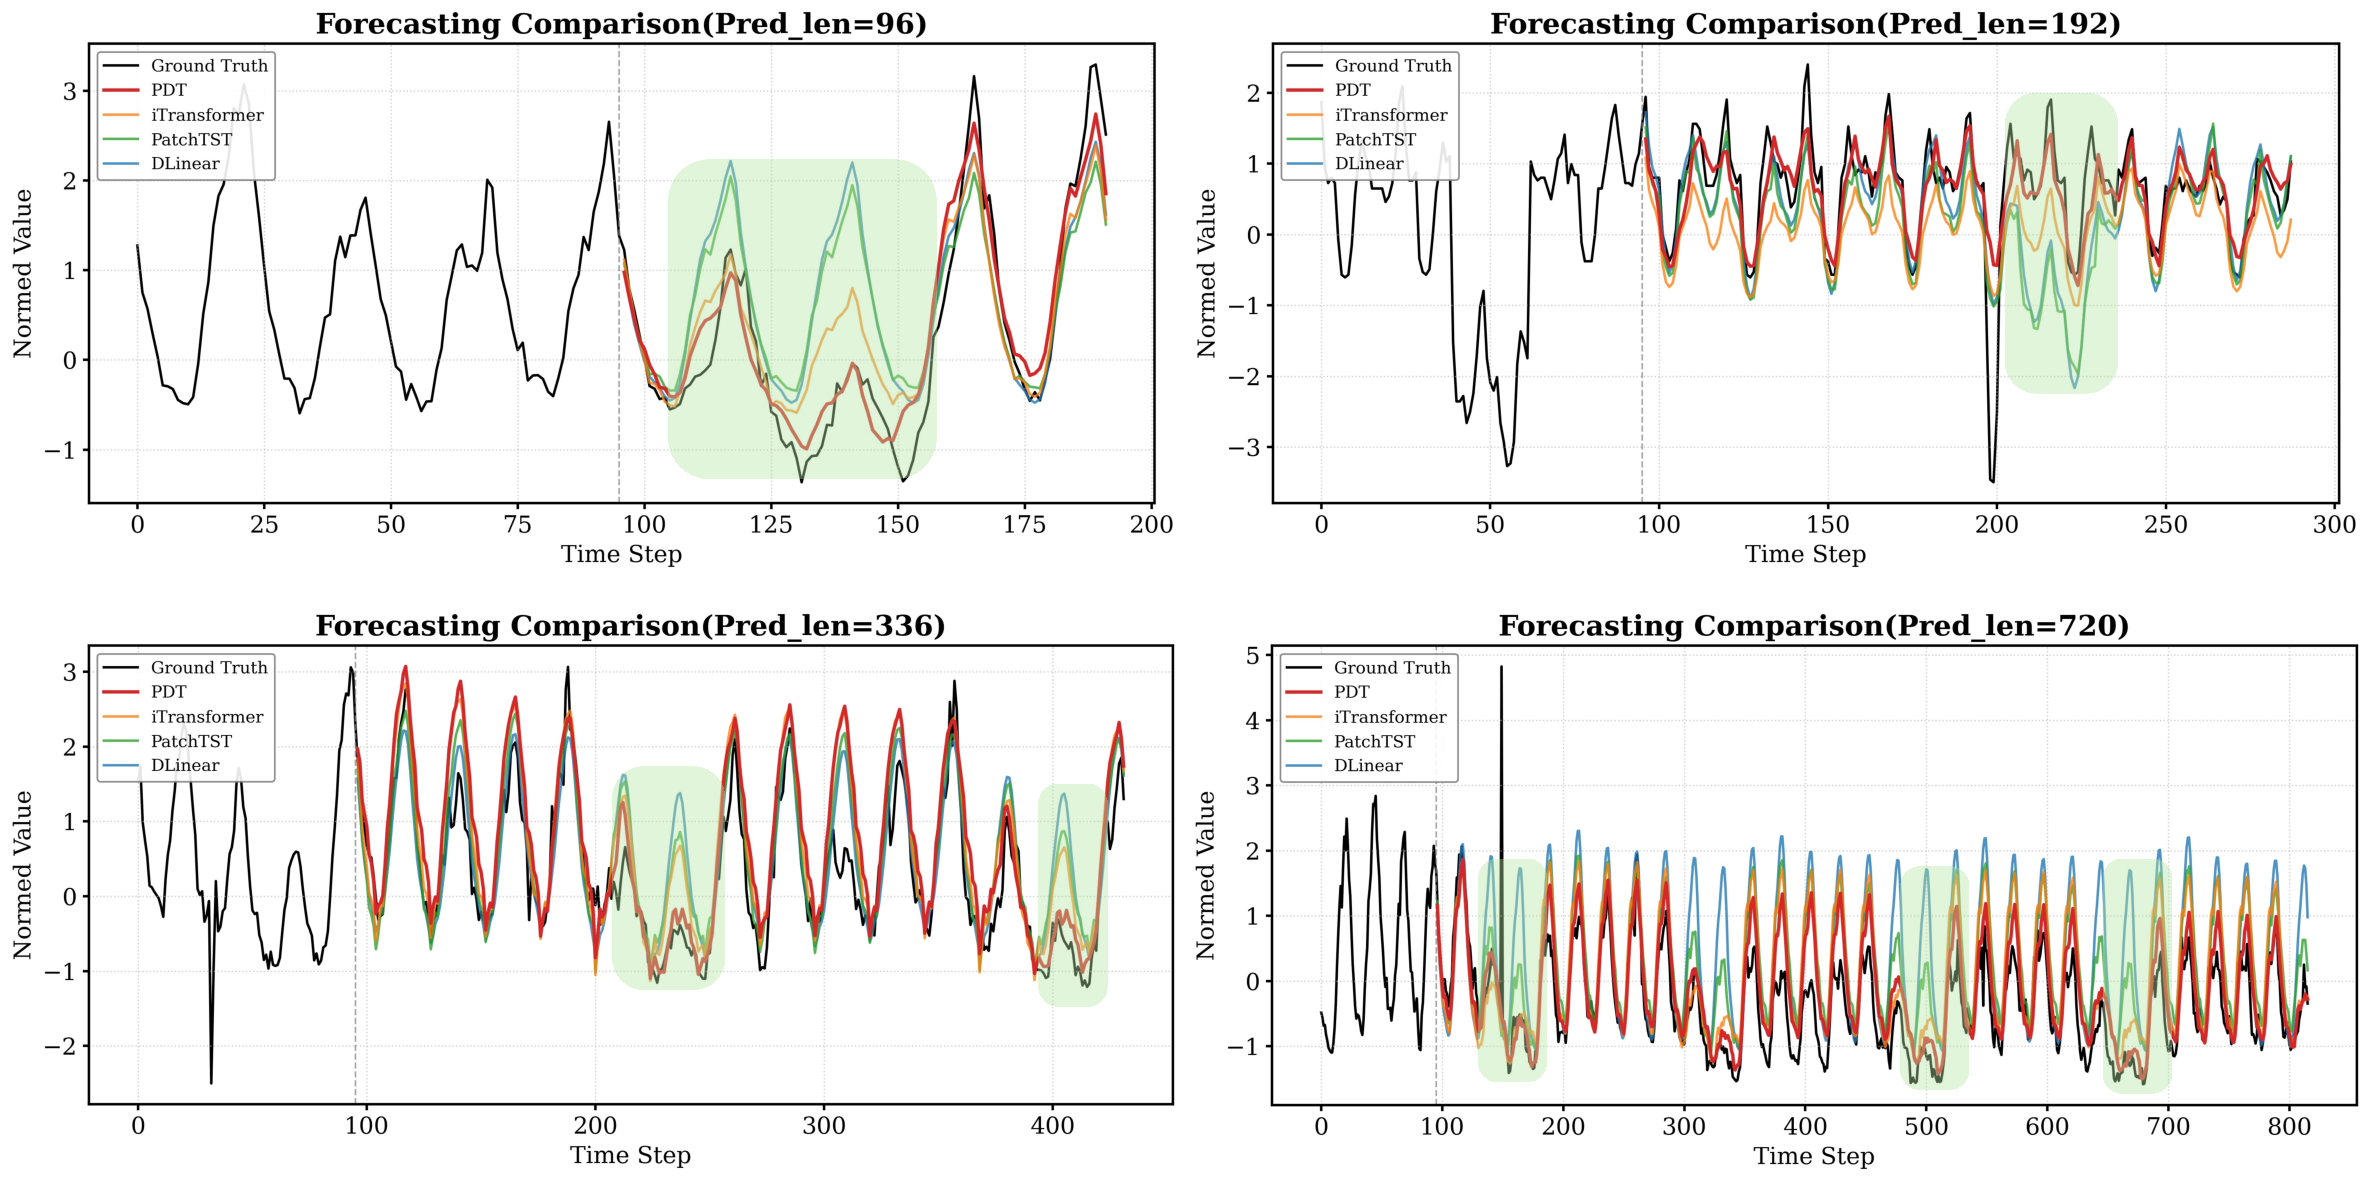
\includegraphics[width=1.0\linewidth]{visual.pdf}
    \caption{\textbf{Visualization of PDT and baselines in different horizons.} The obvious performance gap is highlighted in shallow green.
    }\label{fig:visual}
\end{figure}


\subsection{Ablation Studies}

To rigorously assess the contribution of each component, we conducted ablation experiments on the Electricity, Weather, and ETTh1 datasets. We fixed the look-back window at $L=96$ and evaluated performance across horizons $T \in \{96, 192, 336, 720\}$. In addition to MSE and MAE, we report MACs(Multiply–Accumulate Operations) and Max Memory Cost to quantify the accuracy-efficiency trade-off.

\textbf{Predictive Domain Transform.} We construct a variant \textbf{w/o-PDTM} by removing the transform module to operate directly in the time domain. As observed in Table \ref{tab:abl_pdt}, this leads to consistent performance degradation (e.g., $\sim 3.9\%$ MSE increase on ECL) and higher memory consumption. This confirms that PDTM successfully concentrates predictive energy into Top-$K$ components, acting as an effective dimensionality reduction mechanism that enhances both accuracy and memory efficiency.

\textbf{Dual-Route Architecture.} We isolate the parallel pathways to validate their distinct roles: \textbf{P-Linear} (Linear-Route only) and \textbf{P-Encoder} (Encoder-Route only). Results in Table \ref{tab:abl_pdt} show that \textbf{P-Linear} suffers from severe underfitting on high-dimensional datasets (MSE increases by $22.3\%$ on ECL), proving that simple extrapolation is insufficient for complex correlations. Conversely, \textbf{P-Encoder} degrades in long-term forecasting due to potential overfitting. The full PDT combines the robustness of linear trend extrapolation with the capacity of non-linear encoding, achieving optimal performance without substantial computational overhead.

\textbf{MCD Strategy.} We compare the proposed strategy against three ablation variants: \textbf{PDT-CI} (Channel-Independent), \textbf{PDT-CD} (Channel-Dependent), and \textbf{PDT-Att} (Full-Attention $QK^\top$). As observed in Table \ref{tab:abl_mcd}, \textbf{PDT-CI} incurs high errors in high-dimensional dataset by ignoring dependencies(e.g., $\sim 12.4\%$ MSE increase on ECL), while \textbf{PDT-CD} underperforms due to noise introduction from irrelevant channels(e.g., $\sim 3.8\%$ MSE increase on ECL). Crucially, \textbf{PDT-Att} drastically increases MACs and memory usage while yielding lower accuracy than our method. This validates that the MCD strategy, implemented via lightweight Linear Attention, achieves a superior balance between selective information fusion and computational cost. Moreover, the data reveals a clear trend: as the variate-dimension increases (ETTh1 $\to$ Weather $\to$ ECL), the impact of the inter-channel interaction module becomes more critical, proving the necessity of optimizing inter-variate interactions in high-dimensional complex environments.


\begin{table*}[!t]
\centering
\caption{Ablation study of PDTM and dual-route on ECL, ETTh1, and Weather datasets.}
\resizebox{\textwidth}{!}{% 自动缩放以适应页面宽度
% 列定义：前两列为索引，后续每4列为一个模型块，中间用竖线隔开
\begin{tabular}{c|c|cccc|cccc|cccc|cccc}
\toprule
\multicolumn{2}{c|}{\textbf{Models}} & \multicolumn{4}{c|}{PDT} & \multicolumn{4}{c|}{w/o PDTM} & \multicolumn{4}{c|}{P-Linear} & \multicolumn{4}{c}{P-Encoder} \\
\midrule
% 下方为 Metric 行，但在图中它通常作为表头的一部分，这里放在数据行上方
\multicolumn{2}{c|}{Metric} & MSE & MAE & MACs (G) & Mem (M) & MSE & MAE & MACs (G) & Mem (M) & MSE & MAE & MACs (G) & Mem (MB) & MSE & MAE & MACs (G) & Mem (M) \\
\midrule

\multirow{5}{*}{ECL} 
& 96  & \best{0.133} & \best{0.222} & 1.790 & 151.420 & 0.137 & 0.228 & 1.790 & 151.350 & 0.179 & 0.267 & 0.270 & 19.620 & 0.135 & 0.225 & 1.790 & 145.220 \\
& 192 & \best{0.149} & \best{0.240} & 2.060 & 144.410 & 0.154 & 0.243 & 2.060 & 182.100 & 0.181 & 0.267 & 0.540 & 51.060 & 0.155 & 0.243 & 2.060 & 133.810 \\
& 336 & \best{0.165} & \best{0.255} & 2.465 & 112.690 & 0.172 & 0.260 & 2.465 & 187.340 & 0.193 & 0.278 & 0.946 & 89.270 & 0.168 & 0.258 & 2.465 & 123.840 \\
& 720 & \best{0.195} & \best{0.281} & 3.546 & 166.200 & 0.204 & 0.288 & 3.546 & 201.910 & 0.231 & 0.309 & 2.027 & 154.270 & 0.198 & 0.284 & 3.546 & 99.180 \\
& Avg & \best{0.160} & \best{0.249} & 2.465 & 143.680 & 0.167 & 0.255 & 2.465 & 180.675 & 0.196 & 0.280 & 0.946 & 78.555 & 0.164 & 0.252 & 2.465 & 125.513 \\
\midrule

\multirow{5}{*}{ETTh1} 
& 96  & \best{0.363} & \best{0.384} & 0.032 & 30.180 & 0.368 & 0.388 & 0.032 & 50.850 & 0.392 & 0.405 & 0.006 & 12.510 & 0.365 & 0.386 & 0.032 & 26.560 \\
& 192 & \best{0.413} & \best{0.414} & 0.038 & 56.900 & 0.425 & 0.422 & 0.038 & 56.730 & 0.430 & 0.425 & 0.012 & 33.080 & 0.415 & 0.416 & 0.038 & 29.810 \\
& 336 & \best{0.453} & \best{0.437} & 0.046 & 61.670 & 0.454 & 0.440 & 0.046 & 40.970 & 0.462 & 0.443 & 0.021 & 41.200 & 0.463 & 0.443 & 0.046 & 55.640 \\
& 720 & \best{0.461} & \best{0.464} & 0.070 & 87.740 & 0.472 & 0.471 & 0.070 & 129.760 & 0.461 & 0.465 & 0.044 & 80.280 & 0.472 & 0.471 & 0.070 & 68.310 \\
& Avg & \best{0.423} & \best{0.425} & 0.046 & 59.123 & 0.429 & 0.430 & 0.046 & 69.578 & 0.436 & 0.434 & 0.021 & 41.768 & 0.429 & 0.429 & 0.046 & 45.080 \\
\midrule

\multirow{5}{*}{Weather} 
& 96  & \best{0.152} & \best{0.187} & 0.095 & 30.310 & 0.158 & 0.196 & 0.095 & 30.240 & 0.167 & 0.204 & 0.018 & 12.810 & 0.159 & 0.197 & 0.095 & 26.800 \\
& 192 & \best{0.201} & \best{0.236} & 0.113 & 36.730 & 0.210 & 0.242 & 0.113 & 36.550 & 0.212 & 0.246 & 0.035 & 33.560 & 0.208 & 0.243 & 0.113 & 30.130 \\
& 336 & \best{0.259} & \best{0.279} & 0.139 & 41.490 & 0.266 & 0.284 & 0.139 & 41.530 & 0.265 & 0.284 & 0.062 & 41.930 & 0.263 & 0.283 & 0.139 & 56.090 \\
& 720 & \best{0.338} & \best{0.332} & 0.210 & 87.450 & 0.348 & 0.339 & 0.210 & 126.750 & 0.345 & 0.337 & 0.133 & 81.470 & 0.349 & 0.344 & 0.210 & 69.990 \\
& Avg & \best{0.237} & \best{0.259} & 0.139 & 48.995 & 0.245 & 0.265 & 0.139 & 58.768 & 0.247 & 0.268 & 0.062 & 42.443 & 0.245 & 0.267 & 0.139 & 45.753 \\
\bottomrule
\end{tabular}
}
\label{tab:abl_pdt} 
\end{table*}

\begin{table*}[!t]
\centering
\caption{Ablation study of MCD on ECL, ETTh1, and Weather datasets.}
\resizebox{\textwidth}{!}{% 自动缩放
\begin{tabular}{c|c|cccc|cccc|cccc|cccc}
\toprule
\multicolumn{2}{c|}{\textbf{Models}} & \multicolumn{4}{c|}{PDT} & \multicolumn{4}{c|}{PDT-CI} & \multicolumn{4}{c|}{PDT-CD} & \multicolumn{4}{c}{PDT-Att} \\
\midrule
\multicolumn{2}{c|}{Metric} & MSE & MAE & MACs (G) & Mem (M) & MSE & MAE & MACs (G) & Mem (MB) & MSE & MAE & MACs (G) & Mem (M) & MSE & MAE & MACs (G) & Mem (M) \\
\midrule

\multirow{5}{*}{ECL} 
& 96  & \best{0.133} & \best{0.222} & 1.790 & 151.420 & 0.153 & 0.234 & 1.790 & 79.230 & 0.137 & 0.226 & 1.790 & 51.850 & 0.139 & 0.226 & 2.294 & 165.250 \\
& 192 & \best{0.149} & \best{0.240} & 2.060 & 144.410 & 0.167 & 0.247 & 2.060 & 97.100 & 0.154 & 0.243 & 2.060 & 97.100 & 0.158 & 0.245 & 2.565 & 156.090 \\
& 336 & \best{0.165} & \best{0.255} & 2.465 & 112.690 & 0.182 & 0.263 & 2.465 & 151.640 & 0.171 & 0.260 & 2.465 & 81.670 & 0.174 & 0.263 & 2.970 & 121.260 \\
& 720 & \best{0.195} & \best{0.281} & 3.546 & 166.200 & 0.220 & 0.297 & 3.546 & 207.540 & 0.205 & 0.290 & 3.546 & 207.540 & 0.199 & 0.288 & 4.051 & 212.370 \\
& Avg & \best{0.160} & \best{0.249} & 2.465 & 143.680 & 0.180 & 0.260 & 2.465 & 133.878 & 0.166 & 0.255 & 2.465 & 109.540 & 0.167 & 0.255 & 2.970 & 163.743 \\
\midrule

\multirow{5}{*}{ETTh1} 
& 96  & \best{0.363} & \best{0.384} & 0.032 & 30.180 & 0.367 & 0.386 & 0.032 & 30.180 & 0.363 & 0.384 & 0.032 & 30.180 & 0.367 & 0.387 & 0.039 & 34.190 \\
& 192 & \best{0.413} & \best{0.414} & 0.038 & 56.900 & 0.416 & 0.416 & 0.038 & 36.160 & 0.414 & 0.415 & 0.038 & 62.590 & 0.418 & 0.419 & 0.045 & 93.030 \\
& 336 & \best{0.453} & \best{0.437} & 0.046 & 61.670 & 0.460 & 0.442 & 0.046 & 124.500 & 0.458 & 0.441 & 0.046 & 154.710 & 0.461 & 0.440 & 0.054 & 189.930 \\
& 720 & \best{0.461} & \best{0.464} & 0.070 & 87.740 & 0.477 & 0.475 & 0.070 & 56.510 & 0.472 & 0.471 & 0.070 & 100.580 & 0.474 & 0.472 & 0.077 & 148.650 \\
& Avg & \best{0.423} & \best{0.425} & 0.046 & 59.123 & 0.430 & 0.430 & 0.046 & 61.838 & 0.427 & 0.428 & 0.046 & 87.015 & 0.430 & 0.429 & 0.054 & 116.450 \\
\midrule

\multirow{5}{*}{Weather} 
& 96  & \best{0.152} & \best{0.187} & 0.095 & 30.310 & 0.162 & 0.197 & 0.095 & 30.310 & 0.156 & 0.192 & 0.095 & 30.310 & 0.166 & 0.200 & 0.117 & 34.320 \\
& 192 & \best{0.201} & \best{0.236} & 0.113 & 36.730 & 0.208 & 0.240 & 0.113 & 36.730 & 0.204 & 0.239 & 0.113 & 63.160 & 0.209 & 0.242 & 0.135 & 93.590 \\
& 336 & \best{0.259} & \best{0.279} & 0.139 & 41.490 & 0.266 & 0.282 & 0.139 & 125.570 & 0.261 & 0.282 & 0.139 & 155.780 & 0.265 & 0.284 & 0.161 & 190.990 \\
& 720 & \best{0.338} & \best{0.332} & 0.210 & 87.450 & 0.348 & 0.337 & 0.210 & 56.740 & 0.345 & 0.339 & 0.210 & 98.050 & 0.345 & 0.336 & 0.232 & 143.380 \\
& Avg & \best{0.237} & \best{0.259} & 0.139 & 48.995 & 0.246 & 0.264 & 0.139 & 62.338 & 0.242 & 0.263 & 0.139 & 86.825 & 0.246 & 0.265 & 0.161 & 115.570 \\
\bottomrule
\end{tabular}
}
\label{tab:abl_mcd} 
\end{table*}

\section{Analysis}

\subsection{Computational efficiency}
Computational efficiency is a prerequisite for model deployment in resource-constrained environments. We evaluate the trade-off between forecasting performance and resource consumption using \textbf{MACs} (Multiply-Accumulate Operations) and \textbf{Max Memory}.
Figure \ref{fig: efficiency} illustrates the landscape of various models on the \textbf{Weather} dataset ($L=96, T=192$).
\begin{itemize}
    \item \textbf{Linear vs. Transformer:} While Transformer-based models (e.g., Crossformer, PatchTST) generally achieve competitive accuracy, they incur significantly higher computational costs compared to Linear-based model. Notably, iTransformer also proves efficient as it applies attention across variates rather than time steps, benefiting from the dataset's low dimension and MLP-based temporal modeling.
    \item \textbf{PDT Advantage:} Leveraging the lightweight Linear Attention and the energy concentration of the PDTM module, PDT achieves SOTA performance while maintaining the efficiency profile of purely linear models. Specifically, it requires only $334 \text{ MB}$ of memory and $0.28 \text{ G}$ MACs, comparable to the lightweight linear model, yet surpasses them in accuracy.
\end{itemize}

\begin{figure}[t]
    \centering
    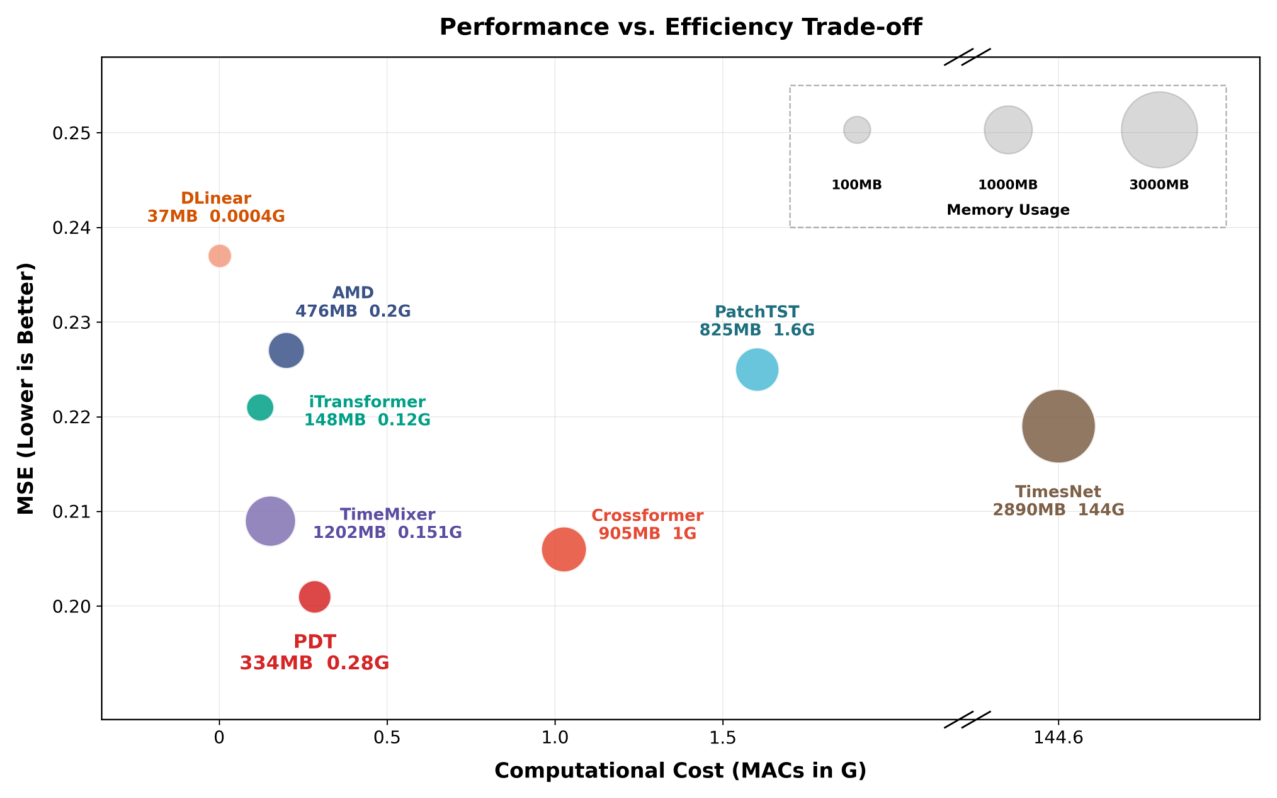
\includegraphics[width=0.5\linewidth]{efficiency.pdf}
    \caption{\textbf{Efficiency-Performance trade-off analysis.} The x-axis represents computational cost (MACs), the y-axis denotes forecasting MSE, and the bubble size corresponds to maximum memory usage.}
    \label{fig: efficiency}
\end{figure}

\subsection{Generality of PDTM}
The proposed \textbf{Predictive Domain Transform Method(PDTM)} is a model-agnostic module designed to enhance feature representation. To verify its generality, we integrate PDTM into the \textbf{iTransformer} backbone (denoted as \textbf{PDT-iTrans}) and compare it against a frequency-domain baseline (\textbf{Freq-iTrans}) which uses Fourier Transform.
As summarized in Table \ref{tab: generality}, incorporating domain transforms consistently improves performance. Notably, PDT-iTrans significantly outperforms Freq-iTrans. On the ECL dataset, PDT-iTrans achieves a $5.4\%$ reduction in MSE compared to $2.6\%$ for Freq-iTrans. Similar trends are observed on ETTh1 and Weather. These results confirm that the learnable, prediction-optimal basis of PDTM offers a more effective feature space than fixed frequency bases, universally boosting the capacity of backbones.

\begin{table*}[!t]
\centering
\caption{Generality of PDTM on iTransformer backbone.}
\resizebox{0.5\textwidth}{!}{
% \setlength{\tabcolsep}{1.5mm}{
% 列定义：前两列(Dataset, Step) | iTransformer(MSE, MAE) | PDT-iTrans(MSE, MAE) | Freq-iTrans(MSE, MAE)
\begin{tabular}{cc|cc|cc|cc}
\toprule
\multicolumn{2}{c|}{Models} & \multicolumn{2}{c|}{iTransformer} & \multicolumn{2}{c|}{PDT-iTrans} & \multicolumn{2}{c}{Freq-iTrans} \\
\midrule
\multicolumn{2}{c|}{Metric} & MSE & MAE & MSE & MAE & MSE & MAE \\ % 图片中Metric行似乎是重复的表头位置，这里按照图片逻辑保留，通常学术表格会合并，这里严格对应图片结构，若不需要可删除此行
\midrule

\multirow{5}{*}{ECL} 
& 96  & 0.148 & 0.240 & 0.140 & 0.228 & 0.146 & 0.234 \\
& 192 & 0.162 & 0.253 & 0.156 & 0.243 & 0.161 & 0.246 \\
& 336 & 0.178 & 0.269 & 0.173 & 0.260 & 0.177 & 0.263 \\
& 720 & 0.225 & 0.317 & 0.206 & 0.288 & 0.210 & 0.291 \\
& Avg & 0.178 & 0.270 & 0.169 & 0.254 & 0.174 & 0.259 \\
\midrule

\multirow{5}{*}{ETTh1} 
& 96  & 0.386 & 0.405 & 0.374 & 0.388 & 0.383 & 0.397 \\
& 192 & 0.441 & 0.436 & 0.426 & 0.417 & 0.433 & 0.426 \\
& 336 & 0.487 & 0.458 & 0.472 & 0.440 & 0.472 & 0.443 \\
& 720 & 0.503 & 0.491 & 0.481 & 0.463 & 0.482 & 0.473 \\
& Avg & 0.454 & 0.448 & 0.438 & 0.427 & 0.442 & 0.434 \\
\midrule

\multirow{5}{*}{Weather} 
& 96  & 0.174 & 0.214 & 0.166 & 0.201 & 0.171 & 0.205 \\
& 192 & 0.221 & 0.254 & 0.212 & 0.245 & 0.219 & 0.250 \\
& 336 & 0.278 & 0.296 & 0.271 & 0.288 & 0.276 & 0.291 \\
& 720 & 0.358 & 0.347 & 0.348 & 0.340 & 0.352 & 0.342 \\
& Avg & 0.258 & 0.278 & 0.250 & 0.269 & 0.255 & 0.272 \\
\bottomrule
\end{tabular}
}
\label{tab: generality}
\end{table*}

\subsection{Architectural Preference across Horizons}
The debate between Linear and Encoder-based architectures is ongoing\cite{zeng2023transformers,li2023revisiting}. We posit that \textit{prediction horizon significantly influences architectural preference}. Leveraging our Dual-Route design, we quantitatively decouple the contributions of the Linear and Encoder routes using the \textbf{Contribution Value (CV)} metric:
\begin{equation}
\begin{aligned}
    CV_{\text{Enc}} &= \frac{\text{MSE}_{\text{P-Linear}} - \text{MSE}_{\text{Full}}}{\text{MSE}_{\text{Full}}} \times 100\% \\
    CV_{\text{Lin}} &= \frac{\text{MSE}_{\text{P-Encoder}} - \text{MSE}_{\text{Full}}}{\text{MSE}_{\text{Full}}} \times 100\%
\end{aligned}
\end{equation}
Specifically, the performance degradation of the P-Linear variant (which masks the Encoder-Route) relative to the full PDT serves as the quantified contribution of the Encoder architecture. Conversely, the degradation of the P-Encoder variant represents the contribution of the Linear architecture.
Experimental results on ECL, ETTh1, and Weather (Fig. \ref{fig: arch_preference}) reveal a distinct evolution in preference: the Encoder architecture ($CV_{\text{Enc}}$) dominates in short-term horizons, while the Linear architecture ($CV_{\text{Lin}}$) becomes pivotal as $T$ extends.
This aligns with theoretical intuition: complex Encoders excel at extracting local, fine-grained details necessary for short-term accuracy, whereas Linear mappings are robust in tracking global trends for long-term forecasting. This finding strongly justifies the necessity of our hybrid Dual-Route architecture.

\begin{figure}[t]
    \centering
    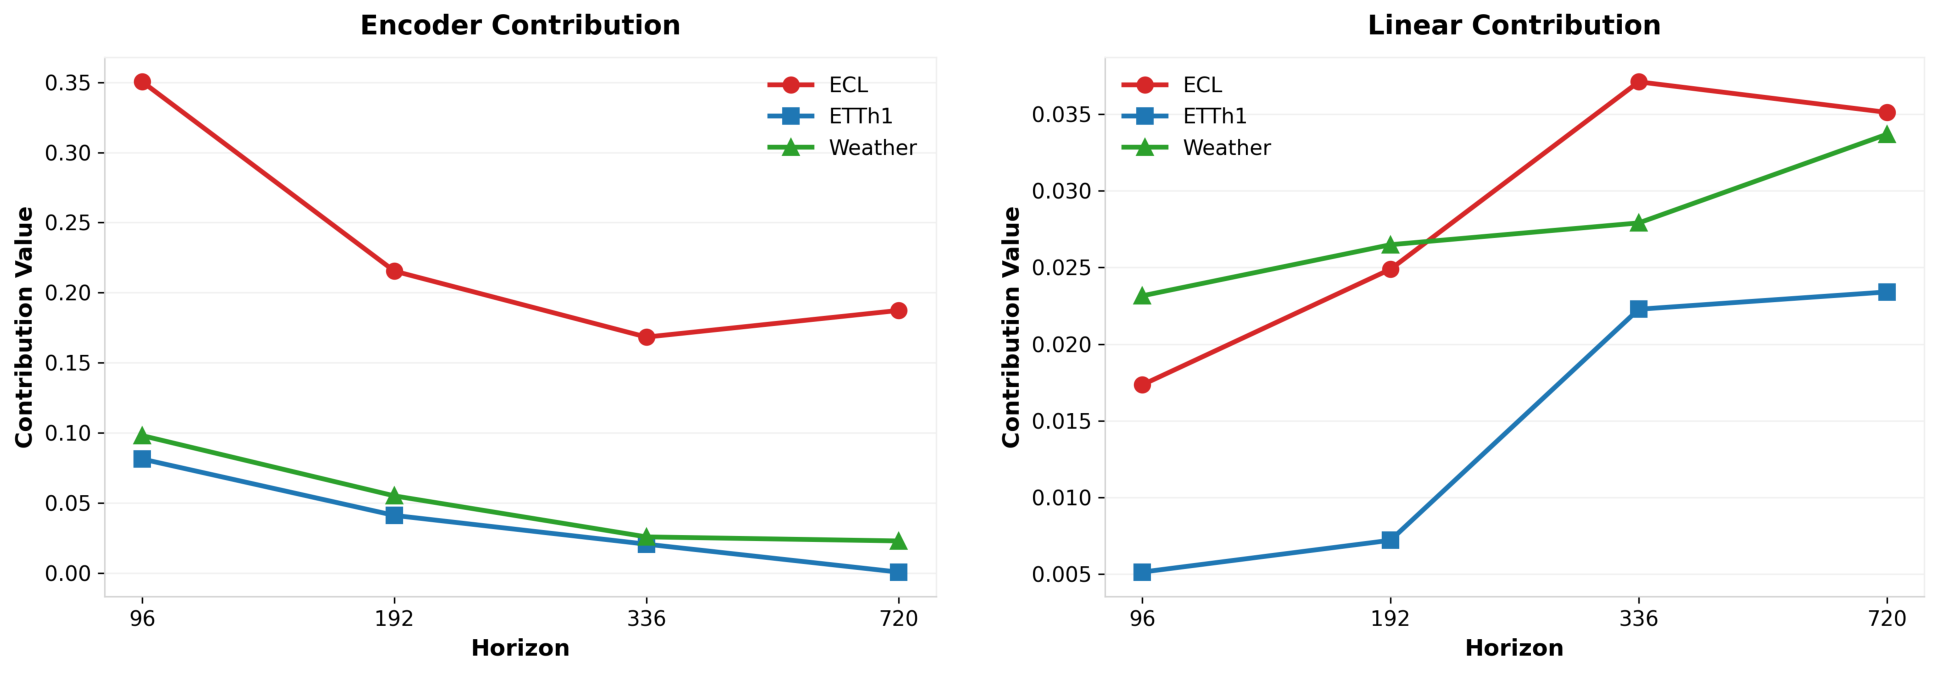
\includegraphics[width=1.0\linewidth]{prefer.pdf}
    \caption{\textbf{Evolution of architectural preference across prediction horizons.}
    \textbf{Left:} The Contribution Value of the Encoder-Route.
    \textbf{Right:} The Contribution Value of the Linear-Route.}
    \label{fig: arch_preference}
\end{figure}

\subsection{Sensitivity to Look-back Window}
A robust model should theoretically benefit from the richer information contained in longer look-back windows ($L$)\cite{box1968some}. However, many existing models degrade as $L$ increases due to noise overfitting\cite{zeng2023transformers}.
We evaluate PDT on Weather and ETTm1 datasets with $L \in \{48,72,96,120,192,336\}$. As shown in Fig. \ref{fig: lookback}, the forecasting accuracy of PDT improves consistently as $L$ increases across all prediction horizons. This consistent improvement demonstrates that the domain transform and the dual-route design effectively mitigate noise, enabling the model to exploit long-range dependencies for precise temporal modeling.

\begin{figure}[t]
    \centering
    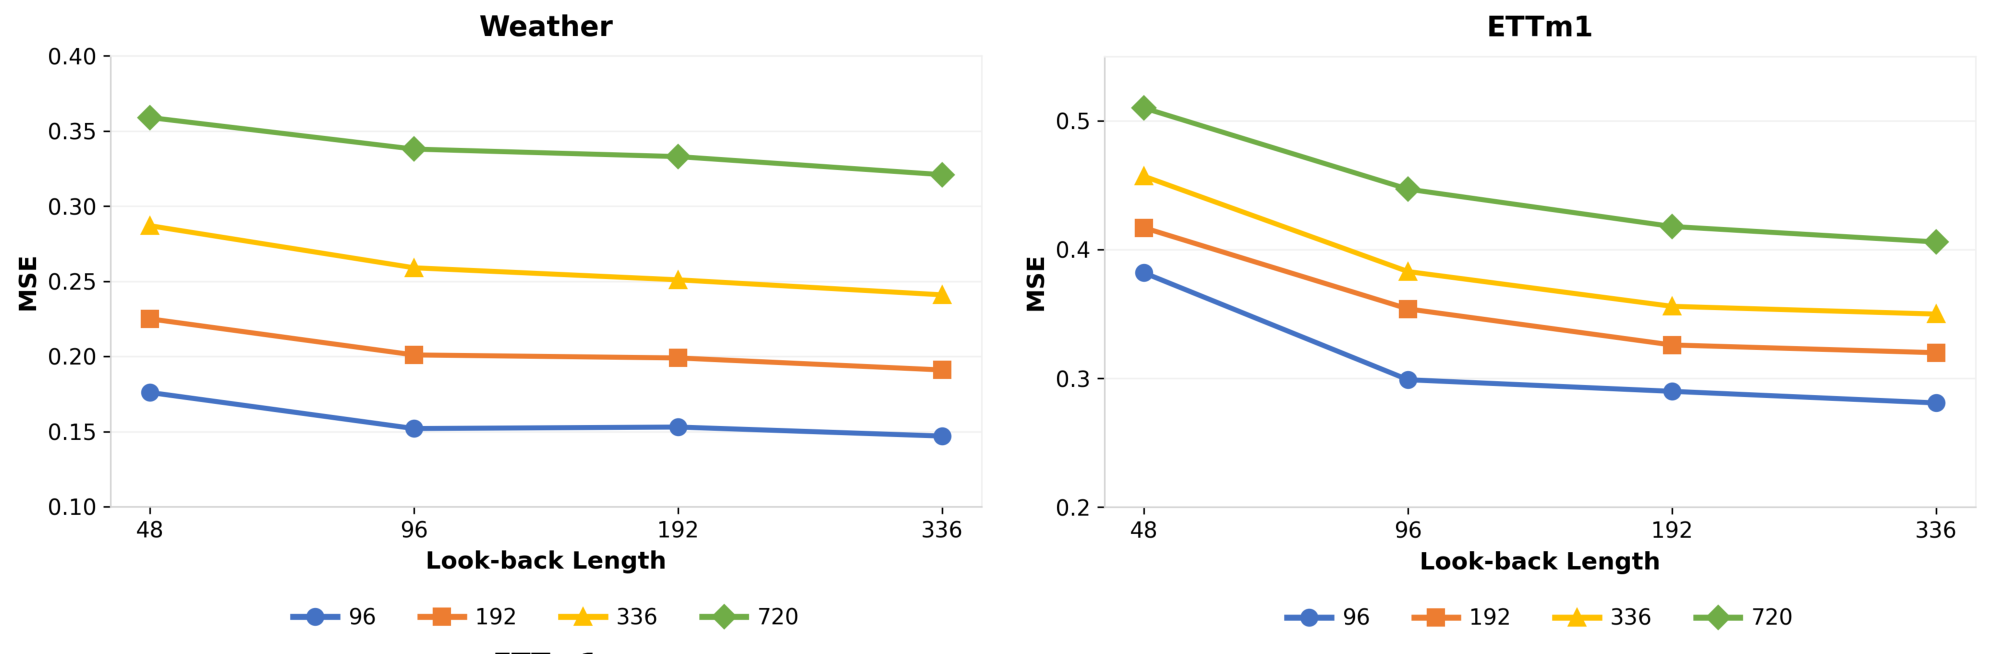
\includegraphics[width=1.0\linewidth]{lookback.pdf}
    \caption{\textbf{Impact of look-back window length on forecasting performance.} The experiments are performed on Weather and ETTm1 datasets with the look-back window $L$ varying from $48$ to $336$.}
    \label{fig: lookback}
\end{figure}

\subsection{Analysis of Series Representation}
We visualize the feature representations learned by the Encoder-Route to validate the effectiveness of the Masked Channel Dependent (MCD) strategy. We compute the cosine similarity matrix of the latent context vectors from the final Encoder layer and compare it with the ground truth correlation matrix of future series. Furthermore, we performed the same visualization for the PDT-CD variant (w/o Mask) to validate the effectiveness of the mask.
As visualized in Fig. \ref{fig: representation}:
\begin{itemize}
    \item \textbf{Accurate Modeling:} The correlation matrix of PDT Fig. \ref{fig: representation}(b) closely aligns with the ground truth Fig. \ref{fig: representation}(a), indicating that the model captures intrinsic inter-variate dependencies.
    \item \textbf{Effect of Masking:} Compared to the PDT-CD variant without masking Fig. \ref{fig: representation}(c), PDT exhibits a sparser and more focused correlation pattern. This confirms that the MCD strategy effectively filters out irrelevant inter-channel noise, guiding the model to focus on meaningful couplings.
\end{itemize}

\begin{figure}[t]
    \centering
    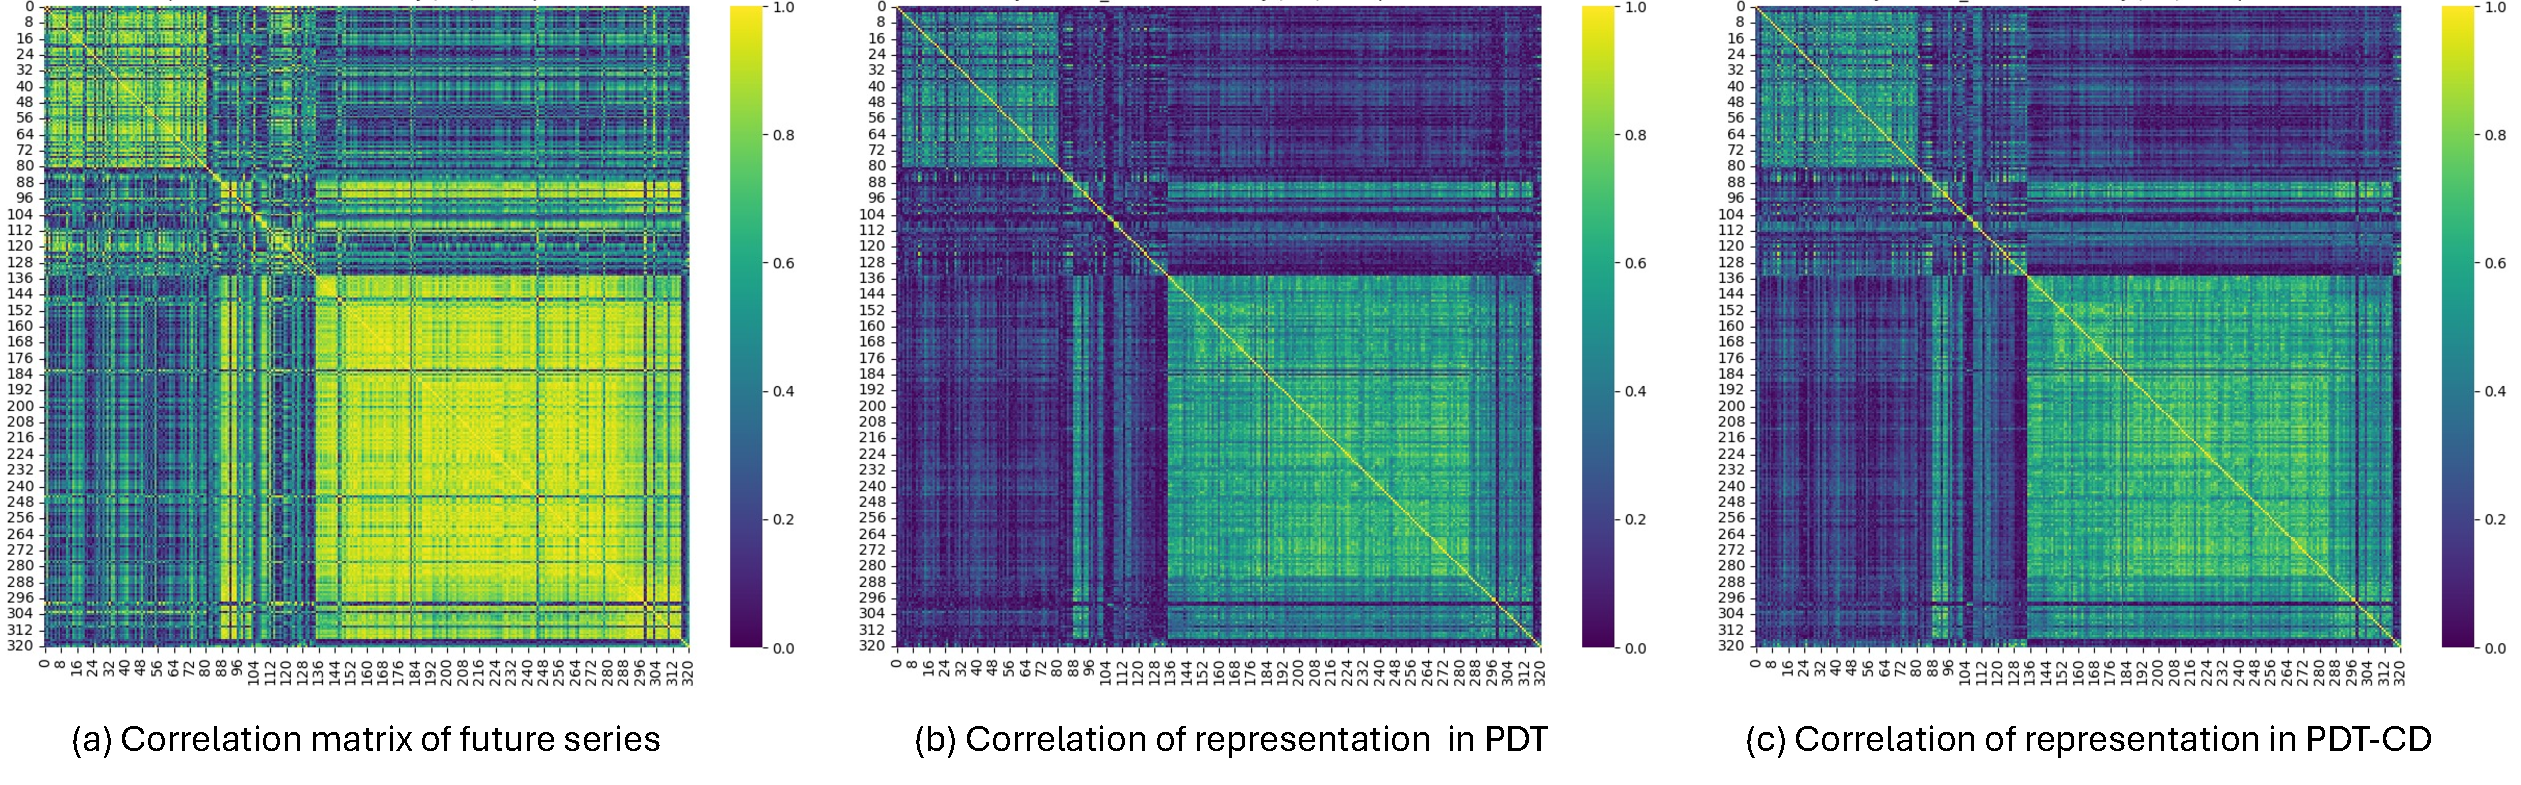
\includegraphics[width=1.0\linewidth]{representation.pdf}
    \caption{\textbf{Visualization of learned feature representations on ECL dataset.} 
    \textbf{(a)} Ground truth correlation matrix of future series. 
    \textbf{(b)} Correlation matrix of representations learned by \textbf{PDT}. 
    \textbf{(c)} Correlation matrix of representations learned by the variant \textbf{PDT-CD} (w/o Mask).
    }
    \label{fig: representation}
\end{figure}



\section{Conclusion}

In this paper, we presented PDT, a novel framework that reconciles the inherent conflict between computational efficiency and representation capacity in multivariate time-series forecasting. 
Central to our approach is the Predictive Domain Transform Method (PDTM), a data-adaptive mechanism that projects series into a prediction-optimal latent space. By exploiting the energy concentration property, PDTM enables a Dual-Route architecture that efficiently extrapolates trends via dominant components while capturing complex residuals through a non-linear encoder.
Furthermore, we addressed the dilemma of channel dependency modeling by introducing the Masked Channel Dependent (MCD) strategy. Implemented via a lightweight Linear Attention, MCD achieves selective feature fusion, effectively suppressing noise from irrelevant variates while preserving critical inter-series couplings. 
Extensive experiments on diverse real-world benchmarks demonstrate that PDT establishes new state-of-the-art performance, validating that a rigorously designed linear backbone, augmented by optimal domain transformation, is sufficient to capture complex temporal dynamics.

\textbf{Limitations and Future Work.} Despite its promising results, several avenues remain for improvement. First, the initialization of the PDTM basis relies on offline statistics from the training set; while we introduce learnable adaptation, the model may still face challenges in streaming scenarios with rapid distribution shifting. Second, the selection of the hyperparameter $K$ (Top-K components) currently relies on empirical validation, lacking a fully adaptive selection mechanism.
Future work will focus on two directions: (1) developing online adaptation algorithms for the transform basis to handle non-stationary distributions in real-time; and (2) extending the prediction-optimal domain concept to general time-series representation learning, paving the way for constructing Foundation Models with strong cross-domain transferability.


\section*{CRediT authorship contribution statement}
\indent \textbf{Chenhao Ying:} Writing – original draft, Writing - review \& editing, Visualization, Validation, Supervision, Software, Resources, Project administration, Methodology, Investigation. \textbf{Jiangang Lu:} Writing - review \& editing, Conceptualization.

\section*{Declaration of Competing Interest}
\indent The authors declare that they have no known competing financial interests or personal relationships that could have appeared to influence the work reported in this paper.

\section*{Data availability}
Data will be made available on request.

\section*{Acknowledgments}
This work was supported in part by the National Natural Science Foundation of China under Grant 62293504, 62293500, and in part by Zhejiang Province Science and Technology Plan Project under Grant 2025C01091.










%% The Appendices part is started with the command \appendix;
%% appendix sections are then done as normal sections
% \appendix
% \section{Example Appendix Section}
% \label{app1}

% Appendix text.

%% For citations use: 
%%       \cite{<label>} ==> [1]

%%
% Example citation, See \cite{lamport94}.

%% If you have bib database file and want bibtex to generate the
%% bibitems, please use
%%
 \bibliographystyle{elsarticle-num} 
 \bibliography{ref}

%% else use the following coding to input the bibitems directly in the
%% TeX file.

%% Refer following link for more details about bibliography and citations.
%% https://en.wikibooks.org/wiki/LaTeX/Bibliography_Management

% \begin{thebibliography}{00}

% %% For numbered reference style
% %% \bibitem{label}
% %% Text of bibliographic item

% \bibitem{lamport94}
%   Leslie Lamport,
%   \textit{\LaTeX: a document preparation system},
%   Addison Wesley, Massachusetts,
%   2nd edition,
%   1994.

% \end{thebibliography}
\end{document}

\endinput
%%
%% End of file `elsarticle-template-num.tex'.
